% This is the Reed College LaTeX thesis template. Most of the work
% for the document class was done by Sam Noble (SN), as well as this
% template. Later comments etc. by Ben Salzberg (BTS). Additional
% restructuring and APA support by Jess Youngberg (JY).
% Your comments and suggestions are more than welcome; please email
% them to cus@reed.edu
%
% See https://www.reed.edu/cis/help/LaTeX/index.html for help. There are a
% great bunch of help pages there, with notes on
% getting started, bibtex, etc. Go there and read it if you're not
% already familiar with LaTeX.
%
% Any line that starts with a percent symbol is a comment.
% They won't show up in the document, and are useful for notes
% to yourself and explaining commands.
% Commenting also removes a line from the document;
% very handy for troubleshooting problems. -BTS

% As far as I know, this follows the requirements laid out in
% the 2002-2003 Senior Handbook. Ask a librarian to check the
% document before binding. -SN

%%
%% Preamble
%%
% \documentclass{<something>} must begin each LaTeX document
\documentclass[12pt,twoside]{templates/facsothesis}
% Packages are extensions to the basic LaTeX functions. Whatever you
% want to typeset, there is probably a package out there for it.
% Chemistry (chemtex), screenplays, you name it.
% Check out CTAN to see: https://www.ctan.org/
%%
\ifxetex
  \usepackage{polyglossia}
  \setmainlanguage{spanish}
  % Tabla en lugar de cuadro
  \gappto\captionsspanish{\renewcommand{\tablename}{Tabla}
          \renewcommand{\listtablename}{Índice de tablas}}
\else
  \usepackage[spanish,es-tabla]{babel}
\fi
%\usepackage[spanish]{babel}
\usepackage{graphicx,latexsym}
\usepackage{amsmath}
\usepackage{amssymb,amsthm}
\usepackage{longtable,booktabs,setspace}
\usepackage{chemarr} %% Useful for one reaction arrow, useless if you're not a chem major
\usepackage[hyphens]{url}
% Added by CII
%\usepackage{hyperref}
\usepackage[colorlinks = true,
            linkcolor = blue,
            urlcolor  = blue,
            citecolor = blue,
            anchorcolor = blue]{hyperref}
\usepackage{lmodern}
\usepackage{float}
\floatplacement{figure}{H}
% End of CII addition
\usepackage{rotating}
\usepackage{placeins} % para fijar la posición de las tablas con \FloatBarrier


\usepackage[]{natbib}


% Next line commented out by CII
%\usepackage{biblatex}
%\usepackage{natbib}
% Comment out the natbib line above and uncomment the following two lines to use the new
% biblatex-chicago style, for Chicago A. Also make some changes at the end where the
% bibliography is included.
%\usepackage{biblatex-chicago}
%\bibliography{thesis}


% Added by CII (Thanks, Hadley!)
% Use ref for internal links
\renewcommand{\hyperref}[2][???]{\autoref{#1}}
\def\chapterautorefname{Chapter}
\def\sectionautorefname{Section}
\def\subsectionautorefname{Subsection}
% End of CII addition

% Added by CII
\usepackage{caption}
\captionsetup{width=5in}
% End of CII addition

% \usepackage{times} % other fonts are available like times, bookman, charter, palatino

% Syntax highlighting #22

% To pass between YAML and LaTeX the dollar signs are added by CII
\title{ ¿Qué pueden hacer las escuelas para promover actitudes positivas hacia la igualdad de derechos? Las buenas relaciones entre profesores y estudiantes como una oportunidad para disminuir las diferencias en estas actitudes}
\author{Anais Herrera Leighton}
% The month and year that you submit your FINAL draft TO THE LIBRARY (May or December)
\date{Santiago de Chile, 2023}
\division{}
\advisor{Profesor guía: Juan Carlos Castillo}
\institution{Universidad de Chile}
\degree{Tesis para optar al grado de Socióloga y Magíster en Ciencias Sociales}
%If you have two advisors for some reason, you can use the following
% Uncommented out by CII
% End of CII addition

%%% Remember to use the correct department!
\department{}
% if you're writing a thesis in an interdisciplinary major,
% uncomment the line below and change the text as appropriate.
% check the Senior Handbook if unsure.
%\thedivisionof{The Established Interdisciplinary Committee for}
% if you want the approval page to say "Approved for the Committee",
% uncomment the next line
%\approvedforthe{Committee}

% Added by CII
%%% Copied from knitr
%% maxwidth is the original width if it's less than linewidth
%% otherwise use linewidth (to make sure the graphics do not exceed the margin)
\makeatletter
\def\maxwidth{ %
  \ifdim\Gin@nat@width>\linewidth
    \linewidth
  \else
    \Gin@nat@width
  \fi
}
\makeatother

%Added by @MyKo101, code provided by @GerbrichFerdinands

\setlength\parindent{0pt}


% Added by CII

\providecommand{\tightlist}{%
  \setlength{\itemsep}{0pt}\setlength{\parskip}{0pt}}

\Acknowledgements{

}

\Dedication{

}

\Preface{

}

\Abstract{

}

	\usepackage{booktabs}
 \usepackage{longtable}
 \usepackage{array}
 \usepackage{multirow}
 \usepackage{wrapfig}
 \usepackage{float}
 \usepackage{colortbl}
 \usepackage{pdflscape}
 \usepackage{tabu}
 \usepackage{threeparttable}
 \usepackage{threeparttablex}
 \usepackage[normalem]{ulem}
 \usepackage{makecell}
 \usepackage{xcolor}
% End of CII addition
%%
%% End Preamble
%%
%
\let\chaptername\relax
\begin{document}
\bibliographystyle{apalike}
% Everything below added by CII
  \maketitle

\frontmatter % this stuff will be roman-numbered
\pagestyle{empty} % this removes page numbers from the frontmatter



%  \hypersetup{linkcolor=black}
  \setcounter{tocdepth}{1}
  \setlength{\parskip}{0pt}
  \tableofcontents

\setlength\parskip{1em plus 0.1em minus 0.2em}

  \listoftables

  \listoffigures



\mainmatter % here the regular arabic numbering starts
\pagestyle{fancyplain} % turns page numbering back on

\hypertarget{resumen}{%
\chapter*{Resumen}\label{resumen}}
\addcontentsline{toc}{chapter}{Resumen}

En un mundo con altos niveles de desigualdad y crecientes expresiones de intolerancia, se hace fundamental la aprobación de políticas públicas que avancen a garantizar la igualdad de derechos. En sociedades democráticas la promoción de estas políticas depende en parte importante de la opinión de la ciudadanía. Uno de los principales espacios en los que el Estado puede intervenir para promover actitudes positivas hacia la igualdad de derechos es la escuela, por su rol fundamental en la socialización de principios y valores. Diversas investigaciones han indagado en los factores asociados a las actitudes hacia la igualdad de derechos de los jóvenes en edad escolar, orientándose en dos líneas: una relacionada con características y experiencias individuales de los estudiantes, y otra enfocada en características y prácticas de la escuela a la que asisten. La presente investigación pretende aportar a estas líneas de estudio incorporando ambas teorías en un modelo estadístico para evaluar si alguna de las características de la escuela (señaladas frecuentemente en investigaciones anteriores) posee la capacidad de disminuir las diferencias individuales en las actitudes hacia la igualdad de derechos. Para ello se estiman regresiones multinivel utilizando datos del Estudio Internacional sobre Educación Cívica y Ciudadana (ICCS) 2016 de 3.920 estudiantes de 8°básico de 166 escuelas chilenas. Los resultados indican que las buenas relaciones entre estudiantes y profesores son capaces de disminuir el efecto del sexo y el nivel de conocimiento cívico en dos de las tres dimensiones de las actitudes hacia la igualdad de derechas analizadas en el estudio.

\textbf{Palabras clave:} \emph{``formación ciudadana''}, \emph{``educación cívica''}, \emph{``igualdad de derechos''}, \emph{``clima escolar''}, \emph{``jóvenes''}.

\hypertarget{introducciuxf3n}{%
\chapter{Introducción}\label{introducciuxf3n}}

La igualdad de derechos es uno de los principios fundamentales de todo sistema democrático, pudiéndose establecer a la vez como un punto de partida y un objetivo de estos (Vila, 2008). Sin embargo, las democracias latinoamericanas y caribeñas aún presentan grandes desafíos en términos de la inclusión de grupos sociales subalternos, lo que se expresa en la mantención de desigualdades sociales, políticas y económicas (Burchardt, 2008; Bárcena et al.~2016) y en el aumento de los delitos de odio por motivos de sexo, religión, orientación sexual y otras condiciones sociales (Organización de los Estados Americanos, 2013). El problema es de tal magnitud que la Comisión Económica para América Latina y el Caribe (CEPAL) ha definido a Latinoamérica como la región más desigual del mundo (Abramo, 2017; CEPAL, 2017), y no sólo por las desigualdades socioeconómicas, sino también porque no se ha logrado que toda la población goce efectivamente de los derechos consagrados en la Declaración Universal de Derechos Humanos (Bárcena et al.~2016).

Los altos niveles de desigualdad presentes en países como Chile nos enfrentan a un panorama doblemente preocupante. Por un lado, las desigualdades perpetúan diferencias en el respeto y la dignidad con que se trata a las distintas personas (Conde, 2014). Estas diferencias en el trato conllevan el surgimiento de prácticas discriminatorias hacia grupos sociales desfavorecidos (Araujo, 2013), como las personas de niveles socioeconómicos bajos, las mujeres, los migrantes, los pertenecientes a grupos étnicos y los homosexuales. En otras palabras, ``(\ldots) los actos de discriminación tienen raíces socioculturales influidas por intereses de grupos que sustentan el poder económico, político y social, cuya concentración de poder se asienta en la desigualdad social y la profundiza.'' (Conde, 2014, p.4). Por otro lado, los altos niveles de desigualdad constituyen una amenaza para el desarrollo sostenible de los países, dificultando el progreso económico, debilitando la democracia y poniendo en peligro la cohesión social (PNUD, 2017). Así, se ha llegado a postular que la desigualdad amenaza incluso la sobrevivencia de las sociedades como tales, debido a que la igualdad es un requisito necesario para que todos puedan reconocerse como parte de la misma sociedad (Garretón, 2015).

La teoría propuesta por Axel Honneth acerca de la justicia social permite ilustrar de buen modo como se entremezclan estas problemáticas de desigualdad, discriminación (o, en sus palabras, menosprecio) y desarrollo de una democracia sostenible con la necesidad de promover la igualdad de derechos. El autor señala que ``la concesión de derechos sociales y la redistribución que la acompaña cumplen la función normativa de conceder a cada uno de los ciudadanos la oportunidad real de participar en el proceso democrático de construcción pública de la comunidad de derecho.'' (Honneth, 2010, p.41) y, en este sentido, plantea que

\begin{quote}
``la misma lucha por la redistribución (\ldots) se halla anclada en una lucha por el reconocimiento: representa un conflicto alrededor de las jerarquías de valores socialmente institucionalizadas que regulan que grupo social tiene derecho a exigir legítimamente -es decir, en función de su estatus y la apreciación de que disfruta- un cierto grado de bienes materiales. En pocas palabras, se trata de una lucha alrededor de la definición cultural de aquello que hace que una actividad social sea socialmente necesaria y valiosa.'' (Honneth, 2010, p.43).
\end{quote}

Así, el autor propone que redistribución y reconocimiento son demandas mutuamente incluyentes, las cuales tienen como horizonte problematizar que aquellos valores socialmente institucionalizados debiesen concederse transversalmente a toda la comunidad. En las sociedades actuales, parte importante de los valores socialmente institucionalizados refieren a los Derechos Humanos, pero en América Latina aún hay sectores de la población que no gozan efectivamente de estos derechos (Bárcena et al.~2016).

Este panorama revela la urgencia de que se promuevan leyes y políticas públicas que garanticen la igualdad de derechos, un principio democrático que sienta las bases del respeto a los Derechos Humanos, para terminar con la discriminación y formar una sociedad donde todos se reconozcan mutuamente. En países democráticos como Chile la promoción de leyes que se orienten en este sentido dependerá, en buena medida, del apoyo de la ciudadanía hacia la igualdad de derechos.

El fomento de políticas públicas que avancen a garantizar la igualdad y la promoción de actitudes positivas hacia la igualdad de derechos entre la ciudadanía son horizontes de organismos internacionales como la Organización de las Naciones Unidas (ONU), frente a los cuales la educación se sitúa como un espacio de socialización capaz de influir en los principios y valores de los estudiantes. La socialización escolar se constituye como un espacio estratégico en el cual el Estado puede intervenir para fomentar principios valóricos de la democracia, como la tolerancia, el respeto y la igualdad, debido a que la escuela es el principal espacio de socialización fuera de la familia. Así se propone en el programa Educación para la Ciudadanía Mundial en América Latina y el Caribe, donde se señala que ``En un mundo con crecientes manifestaciones de intolerancia, es crítico que los sistemas educativos equipen a los estudiantes con valores, conocimientos y habilidades que inculquen respeto por los Derechos Humanos.'' (UNESCO, s.f.). Siguiendo esta línea, en los últimos años el Estado chileno ha aumentado sus esfuerzos por incidir en el proceso de socialización política de los jóvenes, proponiendo la implementación de una política pública de Formación Ciudadana que tiene entre sus objetivos de aprendizaje transversal:

\begin{quote}
``Conocer, respetar y defender la igualdad de derechos esenciales de todas las personas, sin distinción de sexo, edad, condición física, etnia, religión o situación económica, y actuar en concordancia con el principio ético que reconoce que todos los seres humanos nacen libres e iguales en dignidad y derechos y, dotados de razón y conciencia, deben comportarse fraternalmente los unos con los otros'' (Ministerio de Educación, 2016a, p.85).
\end{quote}

De este modo, teniendo en consideración que la promoción de políticas que garanticen la igualdad de derechos depende del apoyo que la ciudadanía dé a la misma y que la escuela es un espacio estratégico donde se puede intervenir para promover actitudes positivas hacia la igualdad de derechos, se vuelve relevante analizar los factores que inciden en el proceso de socialización política de dichas actitudes. Enfocar este análisis en jóvenes en edad escolar puede permitir comprender por qué se generan diferencias en las predisposiciones a la igualdad de derechos para grupos desfavorecidos e identificar las prácticas y/o condiciones de la escuela que favorecen una actitud positiva hacia la igualdad de derechos.

Desde los orígenes de la sociología los procesos de socialización han sido un tema de interés (ej. Durkheim {[}1922{]} 2000), por lo que la pregunta sobre los factores que influyen en la socialización de las actitudes hacia la igualdad de derechos entre los jóvenes no es una novedad. La mayoría de los estudios al respecto se ha enfocado en dos tipos de características: las características individuales del estudiante, y las características de la escuela a la que asiste. Por un lado, se ha evidenciado que los recursos socioeconómicos de la familia del estudiante (Miranda, Castillo y Cumsille, 2018), poseer antecedentes migratorios (Miranda et al.~2018), pertenecer al sexo femenino (Miranda et al.~2018; Schulz, Ainley, Cox y Friedman, 2018) y/o el nivel de conocimiento cívico del estudiante (Schulz et al.~2011; Schulz, Ainley, Cox et al.~2016; Schulz y Ainley, 2018) se asocian positivamente con las actitudes hacia la igualdad de derechos para grupos desfavorecidos. En otras palabras, se ha evidenciado que existen diferencias en las actitudes hacia la igualdad de derechos de los jóvenes que se asocian a características personales. Por otro lado, se ha constatado que la apertura a la discusión en el aula (Barber, Torney-Purta y Fennelly, 2010; Schulz y Ainley, 2018), el clima escolar (Caro y Schulz 2012; Schulz y Ainley, 2018) y la composición del aula (Caro y Schulz 2012; Isac, Maslowski, y Van der Werf, 2012) se asocian a actitudes positivas a la igualdad de derechos.

La presente propuesta de investigación busca ser un aporte a estas líneas de estudio, incorporando los dos tipos de características en un modelo que permita evaluar si la relación entre las actitudes hacia la igualdad de derechos y las características de cada estudiante puede ser moderada por alguno de los factores del proceso de socialización en la escuela que han sido analizados anteriormente en otras investigaciones. La motivación principal de este estudio surge de la siguiente reflexión: si tenemos en consideración que existen diferencias individuales en las actitudes hacia la igualdad de derechos, es necesario indagar en cómo podemos terminar con estas diferencias. Como se ha argumentado anteriormente, la escuela es un ambiente especialmente idóneo para la socialización de principios democráticos como la igualdad de derechos. Pero, si bien distintas investigaciones evidencian que existe una asociación entre ciertas características de la escuela y las actitudes hacia la igualdad de derechos de sus estudiantes, casi no existe evidencia que permita discernir si esas características permiten mitigar, potenciar o reproducir las diferencias provocadas por las características individuales. Por lo tanto, este estudio pretende aportar a la comprensión de qué prácticas y/o características de la escuela permiten disminuir o eliminar las diferencias en las actitudes hacia la igualdad de derechos dadas por las características individuales de los estudiantes. En esta línea, se ha formulado la siguiente pregunta y objetivos de investigación:

\textbf{Pregunta de investigación}

\begin{itemize}
\tightlist
\item
  ¿En qué medida características y prácticas de la escuela afectan la relación entre las actitudes hacia la igualdad de derechos de estudiantes en Chile y sus características individuales?
\end{itemize}

\textbf{Objetivo general}

\begin{itemize}
\tightlist
\item
  Evaluar si alguna/s de las características y prácticas de la escuela posee/n la capacidad de disminuir las diferencias en las actitudes hacia la igualdad de derechos de los jóvenes chilenos, producidas por características individuales de los estudiantes.
\end{itemize}

\textbf{Objetivos específicos}

\begin{itemize}
\item
  Establecer en qué medida las actitudes de los jóvenes chilenos hacia la igualdad de derechos se relacionan con características individuales del estudiante (más específicamente, su sexo, sus antecedentes migratorios, su identificación con un grupo étnico, su nivel de conocimiento cívico y sus recursos socioeconómicos).
\item
  Establecer en qué medida las actitudes de los jóvenes chilenos hacia la igualdad de derechos se relacionan con características y prácticas de la escuela a la que asisten (más específicamente, con la apertura a la discusión en el aula, el clima escolar y las características de sus compañeros de curso).
\item
  Identificar cuáles características y prácticas del contexto escolar poseen la capacidad de disminuir el efecto de las características del estudiante sobre sus actitudes hacia la igualdad de derechos.
\end{itemize}

Se espera que realizar una investigación con estas cualidades constituya un aporte a la comprensión de la capacidad que tienen las escuelas para promover actitudes positivas hacia la igualdad de derechos, dando luces sobre qué prácticas se podrían potenciar en los colegios para prevenir las actitudes discriminatorias.

\hypertarget{antecedentes-teuxf3ricos-y-empuxedricos1}{%
\chapter[Antecedentes teóricos y empíricos]{\texorpdfstring{Antecedentes teóricos y empíricos\footnote{Con el objetivo de transparentar como se realizó la revisión bibliográfica, considero pertinente mencionar que la mayoría de la literatura fue encontrada a través del portal de Scopus, Web of Science o Google Scholar. Las palabras claves en la búsqueda fueron ``actitudes''/``attitudes'', ``igualdad''/``equal'' y ``derechos''/``rights''. Adicionalmente se revisaron dos libros recomendados por mi profesor guía: ``Teaching tolerance in a Globalized World.'' y ``Aprendizaje de la ciudadanía. Contextos, experiencias y resultados.''.}}{Antecedentes teóricos y empíricos}}\label{antecedentes-teuxf3ricos-y-empuxedricos1}}

\hypertarget{actitudes-hacia-la-igualdad-de-derechos}{%
\section{Actitudes hacia la igualdad de derechos}\label{actitudes-hacia-la-igualdad-de-derechos}}

\hypertarget{conceptualizaciuxf3n}{%
\subsection{\texorpdfstring{\emph{Conceptualización}}{Conceptualización}}\label{conceptualizaciuxf3n}}

Antes de profundizar en los antecedentes teóricos y empíricos de la investigación sobre actitudes hacia la igualdad de derechos, cabe precisar qué se entenderá como actitudes hacia la igualdad de derechos.

Para ello, es necesario definir en primer lugar cómo se comprenderá la igualdad de derechos. La igualdad de derechos propiamente tal es un concepto de larga data, el cual tomó fuerza en 1789 con la Declaración de los Derechos del Hombre y del Ciudadano a partir de la sentencia ``Los hombres nacen y permanecen libres e iguales en derechos. Las distinciones sociales sólo pueden fundarse en la utilidad común.'' (Artículo 1). Este planteamiento se ha reformulado y profundizado en la Declaración Universal de Derechos Humanos de 1948, que dicta que ``Todos los seres humanos nacen libres e iguales en dignidad y derechos y, dotados como están de razón y conciencia, deben comportarse fraternalmente los unos con los otros.'' (Artículo 1). En la actualidad, este Artículo de la Declaración Universal de Derechos Humanos sigue vigente y, en el marco del derecho internacional, la igualdad y la no discriminación son entendidos como valores universales y/o principios básicos de los Derechos Humanos que suponen el ``(\ldots) reconocimiento universal de que los derechos básicos y las libertades fundamentales son inherentes a todos los seres humanos, inalienables y aplicables en igual medida a todas las personas.'' (ONU, s.f., párr. 2). La relevancia de la igualdad de derechos en la formación ciudadana ha sido destacada en la Declaración de las naciones unidas sobre la Educación y Formación en materia de Derechos Humanos. Los lineamentos trazados por la Organización de Naciones Unidas señalan que dos de los objetivos fundamentales de la formación en materia de Derechos Humanos son:

\begin{quote}
``{[}1{]} Lograr el ejercicio efectivo de todos los Derechos Humanos y promover la tolerancia, la no discriminación y la igualdad; (\ldots) {[}2{]} Contribuir a la prevención de los abusos y las violaciones de los Derechos Humanos y a combatir y erradicar todas las formas de discriminación y racismo, los estereotipos y la incitación al odio y los nefastos prejuicios y actitudes en que se basan.'' (ONU, 2011, p.4)
\end{quote}

Estas ideas constituyen la base de lo que se entenderá por igualdad de derechos en este estudio.

La selección de los derechos que se han considerado relevantes incorporar en el análisis es amplia. Desde la perspectiva de las generaciones de los Derechos Humanos es posible afirmar que ha habido, al menos, tres generaciones de derechos. La primera generación refiere a los derechos civiles y políticos, la segunda abarca los derechos sociales, económicos y culturales, y la tercera generación (conocida habitualmente como derechos de los pueblos o de solidaridad) aborda las demandas por el derecho al desarrollo, al progreso, la autodeterminación, un ambiente sano, la libertad informática y la identidad. Entendiendo que todas estas generaciones de derechos forman parte de los Derechos Humanos ratificados en los tratados internacionales, se ha decidido no excluir ni privilegiar una generación de derechos en particular. De modo que en esta investigación se entenderá la igualdad de derechos en un sentido amplio, es decir, incorporando derechos civiles y políticos, derechos sociales, económicos y culturales, y derechos de los pueblos como el derecho a la identidad y al progreso.

Habiendo delimitado qué se entenderá en este estudio por igualdad de derechos y cuáles son los derechos que serán considerados, se hace necesario especificar cómo se entenderán las ``actitudes''. Como se ha mencionado anteriormente, esta investigación se enfoca en el proceso de socialización política de las actitudes hacia la igualdad de derechos en jóvenes en edad escolar, por lo que se enmarca como parte de una serie de estudios sobre formación cívica y ciudadana. En este sentido, la precisión del término ``actitudes'' se servirá de las definiciones que se han dado a este concepto en el marco de la formación ciudadana. . Según las orientaciones del Mineduc para la elaboración del plan de Formación Ciudadana, la formación ciudadana se puede definir como el ``Proceso formativo continuo que permite que los niños, niñas, jóvenes y adultos desarrollen un conjunto de conocimientos, habilidades y actitudes que resultan fundamentales para la vida en una sociedad democrática.'' (Mineduc, 2016b, p.11), de modo que las actitudes democráticas son uno de los ámbitos de la formación ciudadana. Más específicamente, las bases curriculares del Mineduc dictan que las actitudes se pueden entender como ``Disposiciones aprendidas para responder de un modo favorable o no favorable, incluyendo componentes afectivos, valorativos y cognitivos.'' (Mineduc, 2017, p.11). En el marco de la educación cívica y ciudadana algunas investigaciones han precisado aún más esta definición, señalando que las actitudes son los juicios o evaluaciones respecto a ideas, objetos, personas, situaciones y/o relaciones, por lo que es posible que las personas alberguen al mismo tiempo actitudes contradictorias (Schulz, Fraillon, Ainley, Losito \& Kerr, 2008; Schulz, Ainley, Fraillon, Losito \& Agrusti, 2016). Asimismo, estos dos equipos de investigación han planteado que las actitudes abarcan tanto aspectos específicos que pueden cambiar con el tiempo, como creencias más amplias y arraigadas que tienden a ser constantes durante períodos más largos de tiempo.

Por último, cabe destacar que actualmente los artículos que se refieren a las actitudes hacia la igualdad de derechos suelen abordar la temática bajo el alero del término tolerancia (por ejemplo, las investigaciones que se presentan en el libro ``Teaching tolerance in a Globalized World'' (Sandoval-Hernández, Isac y Miranda, 2018)). Sin embargo, este concepto puede ser un poco impreciso porque permite, al menos, dos interpretaciones distintas. Por un lado, una forma de interpretar este concepto es la adoptada por organizaciones internacionales como la UNESCO y por autores como Axel Honneth. La UNESCO en la Declaración de Principios sobre la Tolerancia establece que ``Ante todo, la tolerancia es una actitud activa de reconocimiento de los Derechos Humanos universales y las libertades fundamentales de los demás.'' (UNESCO, 1995, p.79). En una línea similar, Honneth (2010) plantea que la tolerancia se puede entender como una disposición normativa respecto del otro, la cual adoptamos cuando lo vemos como un sujeto portador de los mismos derechos. Así, es posible plantear que una primera forma de interpretar el concepto ``Tolerancia'' es entendiéndolo como el reconocimiento de los derechos del otro. Por otro lado, interpretaciones más cercanas al sentido común, asocian este término al mero hecho de soportar algo. Una aproximación a esta definición se puede encontrar en la RAE, donde se define como primera acepción de la tolerancia la acción y efecto de tolerar, y las primeras acepciones de tolerar en el mismo diccionario asocian este concepto al llevar con paciencia, resistir, soportar. De este modo, la segunda interpretación del concepto asocia la tolerancia a resistir o soportar algo, aunque nos disguste. En palabras de Beltrán (2004), es posible establecer que la tolerancia usualmente es entendida en dos sentidos, un sentido positivo que implica la aceptación y reconocimiento del otro, y un sentido negativo en el cual se soporta algo que se considera perjuicioso en algún punto. Para evitar esta frecuente confusión producida por el concepto de tolerancia, he preferido utilizar el concepto ``Actitudes hacia la igualdad de derechos'' que, si bien puede ser menos parsimonioso, es mucho más preciso.

\hypertarget{mediciuxf3n}{%
\subsection{\texorpdfstring{\emph{Medición}}{Medición}}\label{mediciuxf3n}}

En relación con la evidencia empírica en torno a esta temática y la forma en que han sido medidas estas actitudes en investigaciones anteriores, se hace relevante destacar que, pese a haber múltiples investigaciones sobre las actitudes hacia la igualdad de derechos y los factores que influyen en estas tanto en población adulta como en jóvenes, estas actitudes no han sido definidas ni medidas de forma unívoca en la literatura. Una parte importante de los estudios se ha centrado en analizar las actitudes hacia la igualdad de derechos para un grupo en particular, como los inmigrantes (Gorodzeisky \& Semyonov 2009; Isac et al.~2012; Huddleston \& Vink, 2015; Villalobos, Treviño, Wyman, \& Béjares, 2018) o los homosexuales (Schwartz, 2010; Skipworth, Garner \& Dettrey, 2010; Perales, Bouma \& Campbell, 2019), mientras que en otras investigaciones se proponen modelos donde se analiza de forma simultánea las actitudes hacia la igualdad de derechos para más de un grupo desfavorecido (Miranda et al.~2018; Miranda \& Castillo, 2018; Schulz \& Ainley, 2018).

No obstante, el estudio de Miranda \& Castillo (2018) ha estudiado en específico cuál es el modelo de medición para las actitudes hacia la igualdad de género, la igualdad de derechos para todos los grupos étnicos y/o raciales, y la igualdad de derechos para los migrantes que permite comparar los resultados entre países. En su investigación utilizaron los datos de los 38 países que participaron en el estudio ICCS 2009 y constataron que las escalas originales no son invariantes. Sin embargo, realizaron algunas modificaciones para incluir en el modelo sólo aquellos indicadores que refieren específicamente a la igualdad de derechos para cada uno de los grupos enunciados, llegando a proponer un modelo de medición que presenta un ajuste adecuado y es invariante entre los 38 países. Cabe destacar que en su modelo de medida estiman las actitudes hacia estos grupos como tres variables latentes diferentes que están correlacionadas entre sí.

En el presente proyecto de investigación se ha decidido medir las actitudes hacia la igualdad de derechos siguiendo el modelo de medida propuesto por Miranda y Castillo (2018), principalmente por dos razones. En primer lugar, debido a que la mayoría de los estudios previos enfoca la medición en un grupo específico, mientras que el modelo de medición propuesto en su estudio permite indagar al mismo tiempo en las actitudes hacia la igualdad de derechos para tres grupos desfavorecidos\footnote{En específico: mujeres, grupos étnicos y raciales, e inmigrantes.}, explicitando la interrelación entre estas tres actitudes. Esta lógica se condice con los objetivos e intereses del presente proyecto de investigación, donde tal como se decide no privilegiar una generación de derechos en particular, se pretende no enfocar el análisis en un grupo desfavorecido en particular. En segundo lugar, debido a que el modelo propuesto por Miranda y Castillo (2018) presenta evidencias de invarianza de medición en 38 países, lo que significa que permite medir el mismo concepto de la misma manera para diferentes grupos (Rutkowski y Svetina 2014; Van De Schoot et al.2015). Esto permitiría que mi estudio sea replicable en otros países, al menos lo que respecta a dos de las tres variables dependientes.

\hypertarget{factores-relacionados-con-las-actitudes-hacia-la-igualdad-de-derechos}{%
\section{Factores relacionados con las actitudes hacia la igualdad de derechos}\label{factores-relacionados-con-las-actitudes-hacia-la-igualdad-de-derechos}}

Dada la relevancia de las actitudes hacia la igualdad de derechos en un mundo con creciente discriminación y con altos niveles de desigualdad, múltiples investigadores ya han estudiado el tema, tanto en población adulta como en jóvenes. En los dos apartados que se presentan a continuación se profundizará en los antecedentes teórico-empíricos de la investigación sobre las actitudes hacia la igualdad de derechos. Si bien algunas de las teorizaciones que se expondrán no refieren al término actitudes hacia la igualdad de derechos propiamente tal, se ha considerado relevante incorporarlas debido a que han sido utilizadas como base teórica en parte importante de las investigaciones sobre actitudes hacia la igualdad de derechos.

\hypertarget{investigaciones-centradas-en-caracteruxedsticas-individuales}{%
\subsection{\texorpdfstring{\emph{Investigaciones centradas en características individuales}}{Investigaciones centradas en características individuales}}\label{investigaciones-centradas-en-caracteruxedsticas-individuales}}

Algunas investigaciones han evidenciado que características identitarias como pertenecer al sexo femenino y tener antecedentes migratorios poseen una relación positiva con las actitudes hacia la igualdad de derechos. Estas asociaciones pueden ser explicadas a partir de una línea de estudios desarrollada por la psicología social, desde la que se plantea que las personas que se encuentran en una posición de desventaja (ej. mujeres, personas de grupos étnicos o raciales y homosexuales) demandan más igualdad que aquellas personas que no se encuentran en dicha posición (ej. hombres, blancos y heterosexuales) (Miranda et al.~2018). Hay múltiples estudios que permiten constatar el efecto de pertenecer al sexo femenino en las actitudes positivas hacia la igualdad de derechos para distintos grupos tradicionalmente desfavorecidos, como migrantes (Isac et al.~2012; Miranda et al.~2018; Barbey et al.~2010; De Groof, Elchardus, Franck \& Kavadias, 2008; Maurissen, Barber \& Claes, 2020; Farkač, Scott \& Šerek; 2020), homosexuales (Schulz, Ainley, Cox et al.~2016; Schulz et al.~2018), mujeres y personas pertenecientes a grupos étnicos (Schulz \& Ainley, 2018; Miranda et al.~2018). En cambio, la investigación acerca del efecto de tener antecedentes migratorios en las actitudes hacia la igualdad de derechos es más escasa. Al respecto, el estudio de Miranda et al.~(2018) ha constatado que tener antecedentes migratorios se asocia de forma positiva con las actitudes hacia la igualdad de género, la igualdad de derechos para grupos étnicos y la igualdad de derechos para los migrantes (aunque la asociación es más fuerte con la igualdad de derechos para los grupos étnicos y los migrantes que con la igualdad de género). Asimismo, la investigación de Schulz \& Ainley (2018) señala que en algunos países tener antecedentes migratorios se asocia positivamente con las actitudes hacia la igualdad de derechos para todos los grupos étnicos. A partir de los desarrollos teóricos previos y la evidencia empírica, es posible aseverar que este tipo de características identitarias ligadas íntimamente con los privilegios que se gozan en la vida cotidiana juegan un rol fundamental en el desarrollo de actitudes positivas hacia la igualdad de derechos.

En consideración de estos antecedentes, se ha decidido incorporar dichas variables en el análisis para evaluar el efecto de pertenecer al sexo femenino y/o tener antecedentes migratorios en las actitudes hacia la igualdad de derechos. Con el objetivo de profundizar en la teoría sobre los efectos de estar en una posición de desventaja se ha decidido incorporar en el análisis la pertenencia o no a un grupo étnico, pese a que no se han encontrado estudios que indaguen en el efecto de esta variable\footnote{Seguir este objetivo podría conducir a la necesidad de incorporar muchas otras características identitarias que reflejan posiciones de desventaja (como la pertenencia a un género no binario, a una identidad LGBTIQ+ o a un grupo racializado), sin embargo esta indagación excedería los objetivos del presente proyecto de investigación.}. En relación con estos puntos, se sostiene como hipótesis que pertenecer al sexo femenino, tener antecedentes migratorios y pertenecer a un grupo étnico son factores que tendrán una asociación positiva con las actitudes hacia la igualdad de derechos.

En el informe de resultados del Estudio Internacional sobre Educación Cívica y Ciudadana (ICCS) del año 2016, citado anteriormente, se ha destacado también la asociación entre el nivel de conocimiento cívico del estudiante y sus actitudes hacia la igualdad de derechos. Más precisamente, se señala que el otro factor que se asocia positivamente con las actitudes hacia la igualdad de derechos para homosexuales en Latinoamérica es el nivel de conocimiento cívico (Schulz, Ainley, Cox et al.~2016). La relevancia del conocimiento cívico ya había sido postulada anteriormente en el informe de resultados de los países Latinoamericanos que participaron en el Estudio Internacional sobre Educación Cívica y Ciudadana (ICCS) del año 2009. En este informe los investigadores plantean que poseer un nivel alto de conocimiento cívico se asocia con tener actitudes más positivas a la tolerancia de la diversidad en el vecindario (Schulz et al.~2011). Asimismo, el estudio de Schulz \& Ainley (2018) ha evidenciado que el nivel de conocimiento cívico se asocia positivamente con las actitudes hacia la igualdad de género y la igualdad de derechos para todos los grupos étnicos y raciales. En consideración de estos antecedentes, se ha decidido incorporar en el análisis el nivel de conocimiento cívico como un predictor de las actitudes hacia la igualdad de derechos, sosteniendo la hipótesis de que ambas variables se asociarán de forma positiva.

Por último, el estudio de Miranda et al.~(2018) da luces sobre otro factor relevante, asociado al modelo de recursos. Esta teoría ha sido ampliamente evaluada en relación con la participación política de los adultos, concluyéndose que dicha participación se asocia positivamente a la posición social del individuo o, más precisamente, a los recursos de los que dispone (educación, ocupación, ingresos y tiempo, entre otros) (Smets \& van Ham, 2013). En el estudio de Miranda et al.~(2018) el análisis de esta teoría ha sido ampliado a una perspectiva intergeneracional, permitiendo examinar en población juvenil los efectos propuestos en el modelo de recursos. A partir de los datos de los 38 países incorporados en el estudio ICCS 2009 se evaluó la transmisión intergeneracional de la desigualdad en la socialización política, según la cual los estudiantes que pertenecen a una familia con más recursos socioeconómicos poseen mejores puntajes en la prueba de conocimiento cívico y actitudes más democráticas. Para ello analizaron de forma diferenciada la relación entre las actitudes hacia la igualdad de derechos y cada una de las variables incorporadas en el estudio que refieren a los recursos socioeconómicos de la familia: nivel educativo más alto de los padres, el estatus ocupacional más alto de los padres y la cantidad de libros que hay en el hogar. Utilizando modelos de ecuaciones estructurales multinivel, concluyeron que los recursos socioeconómicos de la familia de los estudiantes son un factor relevante para explicar las actitudes positivas hacia la igualdad de derechos. En base a este antecedente, se ha decidido incorporar en el presente estudio los recursos socioeconómicos de la familia del estudiante como una variable predictora, diferenciando el efecto de las tres variables enunciadas. Se sostendrá como hipótesis que los recursos socioeconómicos de la familia del estudiante se asociarán de forma positiva con las actitudes hacia la igualdad de derechos.

En suma, a partir de los antecedentes revisados sobre la asociación entre las actitudes hacia la igualdad de derechos y las características del estudiante y su familia, se propone el siguiente modelo teórico:

\newpage

\begin{figure}

{\centering 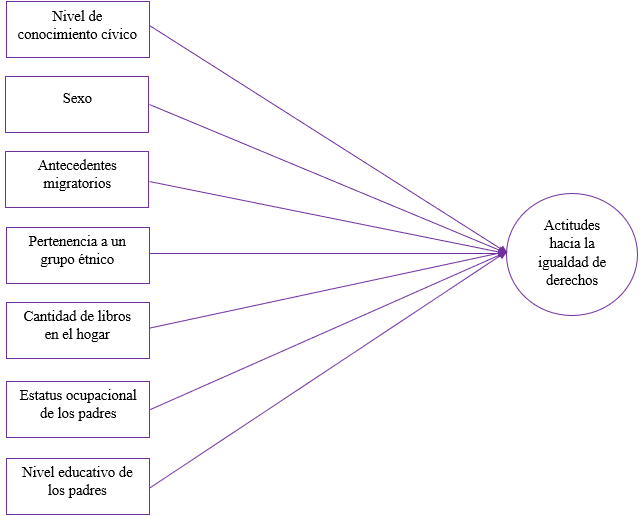
\includegraphics[width=0.9\linewidth]{input/images/modelo_1} 

}

\caption{Modelo teórico sobre la relación entre las características del estudiante y sus actitudes hacia la igualdad de derechos.}\label{fig:unnamed-chunk-2}
\end{figure}

\begin{center}
Fuente: Elaboración propia 

\end{center}

\hypertarget{investigaciones-centradas-en-el-rol-de-las-escuelas}{%
\subsection{\texorpdfstring{\emph{Investigaciones centradas en el rol de las escuelas}}{Investigaciones centradas en el rol de las escuelas}}\label{investigaciones-centradas-en-el-rol-de-las-escuelas}}

Antes de profundizar en los antecedentes teórico-empíricos respecto a las investigaciones centradas en el rol de las escuelas en las actitudes hacia la igualdad de derechos, se hace necesario precisar cómo se ha medido el rol de las escuelas. En investigaciones previas el rol de las escuelas fue medido de diversas formas: a partir de las percepciones de los docentes (ej. Caro \& Schulz, 2012), a partir de las percepciones individuales de los estudiantes (ej. Schulz \& Ainley, 2018), a partir de variables idiosincráticas de nivel escuela{[}\^{}4{]} (ej. Isac et al.~2012) y a partir de las percepciones de los estudiantes tanto a nivel individual como a nivel escuela (ej. Maurissen et al.~2020). {[}\^{}4{]}:Como lo es, por ejemplo, el tamaño de la escuela en metros cuadrados o, en estudios sobre actitudes hacia la igualdad de derechos, la composición en el aula. La revisión bibliográfica abarcará estas diferentes perspectivas, pero se incorporarán al proyecto de investigación los elementos propuestos en la literatura siguiendo los últimos dos enfoques de medición (es decir, utilizando variables idiosincráticas y percepciones de los estudiantes tanto a nivel individual como a nivel escuela\footnote{Estos aspectos relativos a la forma de medición de las variables se presentarán con mayor detalle en el acápite ``Variables''.}).

Al plantearse preguntas sobre el rol de las escuelas, diversas investigaciones sobre equidad en educación incorporan en su análisis la teoría del ``efecto de los compañeros''. Según la cual ``{[}\ldots{]} la composición de los alumnos que comparten un aula-escuela afecta los resultados educacionales obtenidos por dichos alumnos y, en consecuencia, que diferentes agrupaciones de estudiantes producirán logros educativos distintos.'' (Bellei, 2013, p.327). Para explicitar de mejor manera la relación entre el efecto de los compañeros y las actitudes hacia la igualdad de derechos, es posible entrecruzar esta perspectiva con una de las corrientes teóricas sobre la discriminación: la teoría del contacto intergrupal (Allport, 1954). Como se explicó anteriormente, esta teoría plantea que, bajo ciertas condiciones, el contacto entre personas de distintos grupos contribuye a reducir la hostilidad intergrupal. Así, se puede hipotetizar que, si se dan dichas condiciones, el contacto con personas de un grupo diferente al propio promovería actitudes positivas con el exogrupo. Este efecto ha sido evaluado en jóvenes europeos el estudio de Isac et al.~(2012), donde se analizó la relación entre la composición del curso en términos de la proporción de estudiantes inmigrantes en el aula y las actitudes hacia la igualdad de derechos para migrantes, concluyendo que existe una asociación positiva entre ambas variables. Asimismo, la investigación de Sincer, Volman, Veen \& Severiens (2020) sobre estudiantes secundarios de Países Bajos concluye que cuando la composición étnica del aula es diversa, los estudiantes poseen más competencias para lidiar con las diferencias.

Como se puede apreciar, los estudios encontrados que analizan la relación entre las actitudes hacia la igualdad de derechos y la composición del aula refieren a jóvenes de países desarrollados y no se han abordado los posibles efectos de la composición en términos del sexo de los estudiantes. Para aportar evidencias sobre esta relación en un país en vías de desarrollo y sobre la composición en términos del sexo de los estudiantes, el presente estudio indagará en el efecto de la composición del aula en términos de la proporción de niñas, de estudiantes de grupos étnicos y de estudiantes migrantes en la escuela. De este modo se buscará comprender si las actitudes hacia la igualdad de derechos varían en función de las características adscriptivas de los estudiantes que componen el aula y, por ende, del contacto con personas del sexo femenino, pertenecientes a un grupo étnico y/o que han migrado al país. En relación con este punto, se sostendrán tres hipótesis: (1) la proporción de estudiantes en el aula pertenecientes al sexo femenino posee una asociación positiva con las actitudes hacia la igualdad de derechos, (2) la proporción de estudiantes en el aula pertenecientes a un grupo étnico posee una asociación positiva con las actitudes hacia la igualdad de derechos, y (3) la proporción de estudiantes en el aula que posean antecedentes migratorios tendrá una asociación positiva con las actitudes hacia la igualdad de derechos.

Otro eje de análisis relevante en las investigaciones sobre los procesos de socialización refiere al clima escolar. La investigación de Schulz \& Ainley, 2018 ha evidenciado que las actitudes hacia la igualdad de derechos para grupos étnicos y hacia la igualdad de género se asocian significativamente con el clima escolar percibido por el estudiante. Asimismo, la investigación de Maurissen et al.~(2020) ha constatado que hay una asociación positiva entre las actitudes hacia la igualdad para migrantes y el clima escolar percibido por los estudiantes, tanto a nivel individual como a nivel de escuela. Una investigación de una línea de estudios similar a la de la igualdad de derechos ha analizado la asociación entre el clima escolar y la tolerancia a la diversidad en el vecindario utilizando los datos de los países latinoamericanos que participaron en el estudio ICCS 2009, concluyendo que en Chile y Colombia estas variables poseen una relación positiva y significativa, pero con un tamaño efecto bajo (en Chile = 0.09) (Caro \& Schulz, 2012). Sin embargo, existe la posibilidad de que el tamaño de este efecto esté siendo subestimado porque los indicadores que se utilizan para medir el clima escolar son las percepciones de los docentes sobre el clima del aula y los problemas sociales de la escuela. Estos indicadores poseen como problema que la opinión de los docentes podría diferir de la opinión que poseen los estudiantes sobre el clima escolar, siendo poco probable que el grado de tolerancia del estudiante se relacione de forma directa con la percepción del docente sobre el clima escolar. A lo cual se puede añadir que, al tratarse de una encuesta en el marco del espacio laboral, las respuestas de los docentes pueden encontrarse sesgadas por la deseabilidad social. Por ello, en el presente estudio se analizará la relación entre el clima escolar y las actitudes a la igualdad de derechos a partir del set de preguntas sobre el clima en la escuela contestadas por los estudiantes. Al respecto, se sostendrá como hipótesis que en aquellas escuelas en las que los estudiantes perciban un buen clima escolar, se tendrán actitudes más positivas hacia la igualdad de derechos que en otras escuelas.

En una línea de investigación similar, Barber, Torney-Purta y Fennelly (2010), por su parte, y Schulz y Ainley (2018), por otra, han propuesto a partir de sus investigaciones que la apertura a la discusión en el aula genera un ambiente favorable para el desarrollo de actitudes más tolerantes y respetuosas hacia los demás, asociándose positivamente con las actitudes hacia los derechos de los inmigrantes para participar (Barber et al.~2010), las actitudes hacia la igualdad de derechos para grupos étnicos y las actitudes hacia la igualdad de género (Schulz \& Ainley, 2018). Desde la perspectiva de otro destacado investigador de los procesos de socialización política, Campbell (2008), esta asociación se puede explicar a partir de que un clima de aula abierta a la discusión permite una comprensión en mayor profundidad de los principios y prácticas democráticas. Asimismo, siguiendo la teoría democrática deliberativa se supondría que un contexto escolar que estimule la deliberación en el aula fomentaría actitudes más positivas hacia la igualdad de derechos al hacer que los estudiantes compartan sus opiniones con otros que piensan distinto y, con ello, enseñarles a los estudiantes a mostrar más tolerancia hacia la diversidad inherente a nuestra sociedad (Hess 2009; Parker 2003). En consideración de estos antecedentes, se vuelve relevante incluir la percepción de los estudiantes sobre la apertura a la discusión en el aula. En relación con este punto, se sostendrá como hipótesis que en aquellas escuelas en las que los estudiantes perciban un clima más abierto a la discusión en el aula, se tendrán actitudes más positivas hacia la igualdad de derechos que en otras escuelas.

En suma, a partir los antecedentes revisados sobre la asociación entre las características de la escuela y las actitudes hacia la igualdad de derechos, se propone el siguiente modelo teórico:

\begin{figure}

{\centering 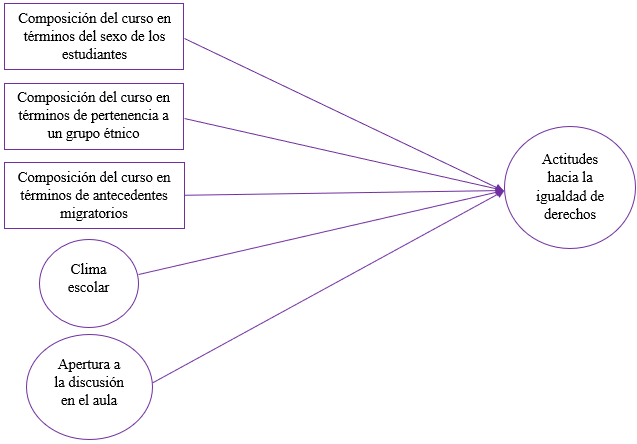
\includegraphics[width=0.9\linewidth]{input/images/modelo_2} 

}

\caption{Modelo teórico sobre la relación entre las características de la escuela y las actitudes hacia la igualdad de derechos}\label{fig:unnamed-chunk-3}
\end{figure}

\begin{center}

Fuente: Elaboración propia 

\end{center}

Por último, como se ha explicado en la introducción, el interés principal de este proyecto de investigación es evaluar si la relación entre las características del estudiante y sus actitudes hacia la igualdad de derechos se puede moderar por alguna/s de las características de la escuela destacadas frecuentemente en las investigaciones previas. Así, se espera aportar a la comprensión de cuáles prácticas y características de las escuelas permiten disminuir las diferencias individuales en las actitudes hacia la igualdad de derechos. Por lo tanto, la hipótesis principal de este estudio es de carácter exploratorio, aunque se sostiene en las múltiples evidencias previas sobre los efectos directos de la composición del aula, la apertura a la discusión y el clima escolar en las actitudes positivas hacia la igualdad de derechos (Isac et al.~2012; Sincer et al.~2020; Barber et al.~2010; Schulz \& Ainley, 2018; Caro \& Schulz, 2012; Maurissen et al.~2020). Además, se tiene como antecedente que el estudio de Isac et al.~(2012) ha evidenciado que en aquellos países donde la composición del aula en términos de proporción de estudiantes migrantes es más diversa, los estudiantes nativos poseen actitudes más positivas hacia la igualdad de derechos que en el resto de los países. Sin embargo, no se poseen más evidencias sobre la interacción entre las características de los estudiantes y las características de la escuela.

Se sostiene como hipótesis que alguna/s de las características de las escuelas (destacadas frecuentemente en investigaciones previas) permitirá moderar el efecto que tienen las características individuales sobre las actitudes hacia la igualdad de derechos. En otras palabras, se espera que alguna de estas características disminuya las diferencias individuales en las actitudes hacia la igualdad de derechos. Para ello, se evaluará el modelo teórico que se presenta a continuación.

\begin{figure}

{\centering 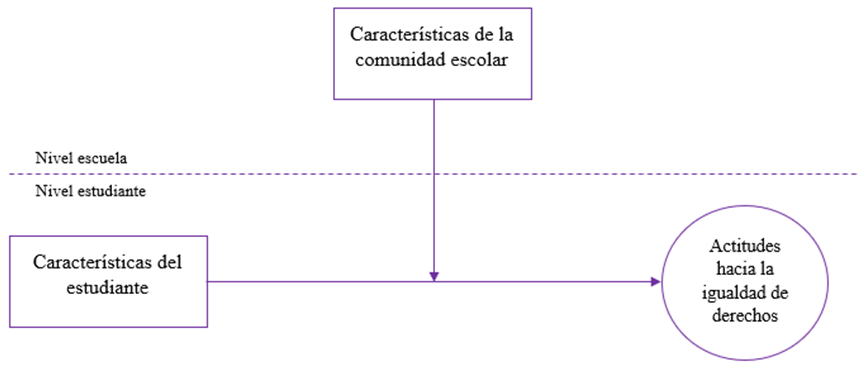
\includegraphics[width=0.8\linewidth]{input/images/modelo_3} 

}

\caption{Modelo teórico sobre la relación entre las características del estudiante y sus actitudes hacia la igualdad de derechos, moderada por las características de la escuela.}\label{fig:unnamed-chunk-4}
\end{figure}

\begin{center}

Fuente: Elaboración propia 

\end{center}

\hypertarget{estrategia-metodoluxf3gica}{%
\chapter{Estrategia Metodológica}\label{estrategia-metodoluxf3gica}}

\hypertarget{datos}{%
\section{Datos}\label{datos}}

Esta investigación utiliza los datos del último estudio Internacional sobre Educación Cívica y Ciudadana (ICCS) de la IEA, el cual consiste en una evaluación estandarizada que permite evaluar cómo las escuelas preparan a sus estudiantes para asumir su rol de ciudadanos, proporcionando evidencia sobre la orientación moral a los Derechos Humanos y la justicia social, el conocimiento cívico y las percepciones sobre el clima escolar de estudiantes de distintas partes del mundo (Schulz, Ainley, Cox et al.~2016). La encuesta fue realizada a una muestra representativa de los estudiantes matriculados en octavo grado en 24 países, siempre que la edad promedio de ese nivel fuera 13,5 años o más (de lo contrario, se define el noveno grado como la población objetivo) (Schulz, Carstens, Losito, \& Fraillon, 2018). En Chile este estudio incorporó a 5.081 estudiantes de 8°básico de 178 escuelas, entre los cuales el 49,3\% se identificó con el sexo femenino y el 50,7\% con el sexo masculino. La muestra incluye establecimientos de todas las regiones, dependencias administrativas y zonas geográficas del país (Agencia de Calidad de la Educación, s.f.). Cabe destacar que se muestreo sólo una clase por escuela, por lo que los datos corresponden a estudiantes que no sólo pertenecen a la misma escuela, sino que comparten en el aula de clases (Schulz, Carstens, Losito, \& Fraillon, 2018). En la presente investigación se trabaja con los datos de 3.920 estudiantes de 166 escuelas, correspondientes a los casos con información completa para las variables de interés en el análisis (es decir, se han excluido todos los casos que tienen un dato perdido en alguna de las variables de interés).

\hypertarget{variables}{%
\section{Variables}\label{variables}}

En esta sección se presentan las variables a utilizar y sus respectivos códigos en la base de datos ICCS.

\hypertarget{indicadores-de-las-actitudes-hacia-la-igualdad-de-derechos}{%
\subsection{\texorpdfstring{\emph{Indicadores de las actitudes hacia la igualdad de derechos}}{Indicadores de las actitudes hacia la igualdad de derechos}}\label{indicadores-de-las-actitudes-hacia-la-igualdad-de-derechos}}

En la encuesta se realiza una serie de preguntas referidas a las actitudes hacia la igualdad de derechos a tres grupos desfavorecidos (mujeres, grupos étnicos o raciales y homosexuales). Este set de preguntas se establece como el objeto central de este estudio. Se estimó un Análisis Factorial Confirmatorio (AFC) para evaluar la bondad de ajuste del modelo de medida de la escala (detalles en Anexo 1), logrando un ajuste adecuado según los criterios propuestos por Brown (2015) al dividirla en las tres dimensiones que se han enunciado: (1) Actitudes hacia la igualdad de derechos entre hombres y mujeres, (2) Actitudes hacia la igualdad de derechos para grupos étnicos o raciales y (3) Actitudes hacia la igualdad de derechos para homosexuales. En consecuencia, se utilizaron tres variables para medir las actitudes de los jóvenes hacia la igualdad de derechos, las cuales fueron generadas utilizando las puntuaciones factoriales estimadas a partir de este AFC.

Como se enuncio en los antecedentes teóricos y empíricos, en términos generales la medición de las actitudes hacia la igualdad de derechos sigue la propuesta de Miranda y Castillo (2018). Más precisamente, se utiliza el modelo de medida propuesto para las actitudes hacia la igualdad de derechos entre hombres y mujeres y hacia la igualdad de derechos para grupos étnicos. Por lo tanto, sólo se incorporan en el análisis los indicadores que refieren específicamente a la igualdad de derechos, pese a que las escalas originales incorporan otros indicadores. Como en dicho artículo no se incorpora un análisis de la escala de actitudes hacia la igualdad de derechos para homosexuales (debido a que es una escala que no estaba en el estudio ICCS 2009), se ha seguido el mismo criterio utilizado por los autores para definir si excluir o no alguno de los indicadores. En consecuencia, se ha decidido no excluir ninguno de los indicadores de dicha escala debido a que al evaluarlos se ha concluido que todos refieren específicamente a la igualdad de derechos y no a otros constructos.

Más específicamente, las actitudes han sido medidas en función del grado de acuerdo con diferentes afirmaciones en una escala de 1 a 4, donde: 1. Muy de acuerdo, 2. De acuerdo, 3. En desacuerdo, 4. Muy en desacuerdo. Para facilitar el análisis, las categorías de respuesta han sido recodificadas de modo que 1 representa ``Muy en desacuerdo'', 2 ``En desacuerdo'', 3 ``De acuerdo'' y 4 ``Muy de acuerdo''. Los indicadores de cada escala y sus códigos se presentan a continuación:

\textbf{Actitudes hacia la igualdad de derechos entre hombres y mujeres}

\begin{itemize}
\item
  Existen diferentes puntos de vista sobre los roles de mujeres y hombres en la sociedad. ¿Cuán de acuerdo o en desacuerdo estás tú con las siguientes declaraciones?

  \begin{itemize}
  \tightlist
  \item
    Los hombres y las mujeres deberían tener las mismas oportunidades de participar en el gobierno. (IS3G24A)
  \item
    Los hombres y las mujeres deberían tener los mismos derechos en todos los aspectos. (IS3G24B)
  \item
    Los hombres y las mujeres deberían recibir el mismo pago cuando están haciendo los mismos los trabajos. (IS3G24E)
  \end{itemize}
\end{itemize}

\textbf{Actitudes hacia la igualdad de derechos para grupos étnicos}

\begin{itemize}
\item
  Existen diferentes puntos de vista sobre los derechos y responsabilidades de los diferentes en la sociedad. ¿Cuán de acuerdo o en desacuerdo estás tú con las siguientes declaraciones?

  \begin{itemize}
  \tightlist
  \item
    En Chile todos los grupos étnicos y raciales deberían tener la misma oportunidad de acceder a una buena educación. (IS3G25A)
  \item
    En Chile todos los grupos étnicos y raciales deberían tener la misma oportunidad de conseguir buenos trabajos. (IS3G25B)
  \item
    Las escuelas deberían enseñar a los estudiantes a respetar a los miembros de todos los grupos étnicos y raciales. (IS3G25C)
  \item
    Los miembros de todos los grupos étnicos y raciales deberían tener los mismos derechos y responsabilidades. (IS3G25E)
  \end{itemize}
\end{itemize}

\textbf{Actitudes hacia la igualdad de derechos para homosexuales}

\begin{itemize}
\item
  ¿En qué medida estás de acuerdo o en desacuerdo con las siguientes afirmaciones respecto a la homosexualidad?

  \begin{itemize}
  \tightlist
  \item
    Las personas del mismo sexo deberían tener derecho a casarse entre sí. (LS3G08A)
  \item
    Dos personas del mismo sexo deberían tener el derecho de adoptar hijos. (LS3G08B)
  \item
    Los homosexuales deberían tener los mismos derechos que los demás ciudadanos. (LS3G08C)
  \item
    Todos los colegios deberían aceptar a homosexuales. (LS3G08D)
  \item
    Los homosexuales deberían tener el derecho de postularse para cualquier cargo político o público. (LS3G08E)
  \end{itemize}
\end{itemize}

\hypertarget{indicadores-de-las-variables-independientes}{%
\subsection{Indicadores de las variables independientes}\label{indicadores-de-las-variables-independientes}}

\hypertarget{nivel-estudiante}{%
\subsubsection{Nivel estudiante}\label{nivel-estudiante}}

\textbf{Nivel de conocimiento cívico (PV1CIV)}

\begin{itemize}
\tightlist
\item
  La variable corresponde al puntaje asignado al nivel de conocimiento cívico del estudiante, como resultado de un procedimiento basado en la teoría de respuesta al ítem para estimar los valores plausibles de conocimiento cívico del estudiante en base a su respuesta a 87 preguntas. Los valores de esta variable varían entre el 0 y el 800, donde un puntaje mayor indica un mayor nivel de conocimiento cívico.
\end{itemize}

\textbf{Sexo (S\_Gender)}

\begin{itemize}
\tightlist
\item
  Esta variable distingue entre hombre (0) y mujer (1).
\end{itemize}

\textbf{Antecedentes migratorios (IS3G04A)}

\begin{itemize}
\tightlist
\item
  Al estudiante se le pregunta en qué país nació (IS3G04A) y en qué países nacieron sus padres (país en qué nació la madre = IS3G04B; país en qué nació el padre = IS3G04C). Haber nacido en Chile fue codificado como 1, y haber nacido en cualquier otro país fue codificado como 0.
\end{itemize}

\textbf{Pertenencia a un grupo étnico (IS3G02BN)}

\begin{itemize}
\tightlist
\item
  Al estudiante se le solicita que escriba las tres palabras que mejor lo describen. Si entre estas palabras el estudiante escribe un pueblo nativo chileno, su respuesta es codificada como ``15202''.
\end{itemize}

\textbf{Recursos socioeconómicos de la familia}

En la encuesta existen tres variables referidas a los recursos socioeconómicos de la familia del estudiante. Como se mencionó anteriormente, se evaluará el efecto de cada variable por separado. Las preguntas y sus categorías de respuesta se presentan a continuación:

\begin{itemize}
\item
  \textbf{\emph{El nivel educativo alcanzado más alto entre los dos padres (S\_HISCED).}} Para construir esta variable al estudiante se le presentan dos preguntas: 1) ¿Cuál es el nivel más alto de educación completado por su madre o tutora?, 2) ¿Cuál es el nivel más alto de educación completado por su padre o tutor? Ambas preguntas tienen las mismas opciones de respuesta: 0) No completo la enseñanza básica, 1) Enseñanza básica, 2) Enseñanza media, 3) Una carrera profesional o técnica, 4) Una carrera universitaria o estudios de posgrado (magister o doctorado). Se compararon las respuestas de los estudiantes a estas dos preguntas y se construyó una nueva variable (S\_HISCED), cuyo valor corresponde al nivel educativo más alto completado por uno de los dos padres (o tutores).
\item
  \textbf{\emph{La ocupación de mayor estatus entre los dos padres (S\_HISEI).}} Para construir esta variable se le presentan cuatro preguntas abiertas al estudiante: 1) ¿Cuál es el trabajo principal de su madre o tutora? (por ejemplo, maestro de escuela secundaria, ayudante de cocina, gerente de ventas), 2) ¿Qué hace tu madre o tutora en su trabajo principal? (por ejemplo, enseña a los estudiantes de secundaria, ayuda al cocinero a preparar las comidas en un restaurante, gestiona un equipo de ventas), 3) ¿Cuál es el trabajo principal de su padre o tutor? (por ejemplo, maestro de escuela secundaria, ayudante de cocina, gerente de ventas), 4) ¿Qué hace tu padre o tutor masculino en su trabajo principal? (por ejemplo, enseña a los estudiantes de secundaria, ayuda al cocinero a preparar las comidas en un restaurante, gestiona un equipo de ventas). El valor asignado a las respuestas de estas preguntas se determina en función de las puntuaciones en el esquema de clasificación ocupacional ISCO-08 y se recodifican a puntuaciones SEI (índice socioeconómico de Duncan). Después de esta recodificación, se compara el puntaje del estatus ocupacional de la madre (o tutora) con el puntaje del estatus ocupacional del padre (o tutor) para crear una nueva variable, cuyo valor corresponde al puntaje del estatus ocupacional más alto entre los dos padres (o tutores). Esta variable será la que se incorporará en el análisis (S\_HISEI).
\item
  \textbf{\emph{La cantidad de libros en el hogar (IS3G11).}} Al estudiante se le pregunta ``¿Aproximadamente cuántos libros hay en tu casa? No cuente revistas, periódicos, historietas, libros electrónicos o sus libros escolares'' y se le presentan 5 categorías de respuesta: 1) Ninguno o muy pocos (0-10 libros), 2) Suficiente para llenar un estante (11-25 libros), 3) Suficiente para llenar dos estantes (26-100 libros), 4) Suficiente para llenar dos estanterías (101-200 libros) y 5) Suficiente para llenar tres o más estanterías (más de 200 libros).
\end{itemize}

\hypertarget{nivel-escuela}{%
\subsubsection{Nivel escuela}\label{nivel-escuela}}

\textbf{Composición del curso en términos de género}

A partir de la pregunta por el sexo de cada estudiante, se creó una variable que representa la proporción de mujeres en el curso. En esta variable el valor 0 indica que en la escuela no estudia ninguna niña, mientras que el valor 1 indica que en la escuela sólo estudian niñas.

\textbf{Composición del curso en términos de antecedentes migratorios}

A partir de las preguntas por los antecedentes migratorios de cada estudiante, se creó una variable que representa la proporción de estudiantes con antecedentes migratorios en el curso. En esta variable el valor 0 indica que en la escuela no estudia nadie con antecedentes migratorios, mientras que el valor 1 indica que en la escuela sólo estudian personas con antecedentes migratorios.

\textbf{Composición del curso en términos de la proporción de estudiantes pertenecientes a un grupo étnico}

A partir de la pregunta por la pertenencia a un grupo étnico, se creó una variable que representa la proporción de estudiantes pertenecientes a un grupo étnico en el curso. En esta variable el valor 0 indica que en la escuela no estudia nadie perteneciente a un grupo étnico, mientras que el valor 1 indica que en la escuela sólo estudian personas pertenecientes a grupos étnicos.

\textbf{Apertura a la discusión en el aula}

Se ha decidido promediar por escuela las respuestas de los estudiantes a cada uno de los indicadores de la escala con el objetivo de obtener una medida que represente de mejor manera la apertura a la discusión en el aula, debido a que las percepciones de cada uno de los estudiantes pueden estar influidas por otros factores (como el compromiso político del joven) (Campbell, 2008). De modo que todos los estudiantes pertenecientes a una misma aula recibirán la misma puntuación en cada uno de los indicadores.

Al ser una variable latente se siguió el mismo procedimiento que con las variables dependientes. En otras palabras, se estimó un AFC para evaluar la bondad de ajuste del modelo de medida de la escala (detalles en Anexo 1), logrando un ajuste adecuado según los criterios propuestos por Brown (2015) al analizarlo como un constructo unidimensional. En función de estos resultados, se utilizó una variable para medir las percepciones de los estudiantes sobre la apertura a la discusión en el aula, siendo esta generada a partir de las puntuaciones factoriales que se pueden estimar en base al modelo de AFC estimado.

En relación con los indicadores de la escala, cabe destacar que al estudiante se le pregunta la frecuencia en qué ocurren determinadas situaciones durante las clases, pidiéndole que escoja entre los siguientes grados de frecuencia: 1) Nunca, 2) Raramente, 3) A veces, 4) A menudo. A continuación se expone la pregunta general y los distintos indicadores, con sus respectivos códigos.

\begin{itemize}
\item
  Cuando se discuten temas políticos o sociales durante las clases regulares, ¿con qué frecuencia suceden las siguientes cosas?

  \begin{itemize}
  \tightlist
  \item
    Los maestros alientan a los estudiantes a tomar sus propias decisiones. (IS3G17A)
  \item
    Los maestros alientan a los estudiantes a expresar sus opiniones. (IS3G17B)
  \item
    Los estudiantes presentan eventos políticos actuales para su discusión en clase. (IS3G17C)
  \item
    Los estudiantes expresan opiniones en clase incluso cuando sus opiniones son diferentes de la mayoría de los otros estudiantes. (IS3G17D)
  \item
    Los maestros alientan a los estudiantes a discutir los problemas con personas que tienen opiniones diferentes. (IS3G17E)
  \item
    Los maestros presentan varios lados de los problemas cuando los explican en clase. (IS3G17F)
  \end{itemize}
\end{itemize}

\textbf{Clima escolar}

En consideración de los argumentos expuestos en la justificación de cómo se medirá la variable apertura a la discusión en el aula, se ha decidido medir el clima escolar siguiendo la misma lógica. En otras palabras, debido a que la percepción del clima escolar de cada estudiante puede estar influida por características individuales y, por ende, puede no representar a cabalidad cómo es el clima escolar de ese colegio, se ha decidido estimar promedios por escuela para las variables de clima escolar.

Respecto a las dimensiones y los indicadores del clima escolar, cabe mencionar que en el cuestionario se realizan dos series de preguntas sobre el clima escolar, una referida a la percepción del estudiante acerca de las relaciones interpersonales en la escuela (tanto entre los profesores y los estudiantes, como entre los estudiantes) y otra enfocada en la vivencia de situaciones de violencia física, emocional y/o verbal en la escuela. La propuesta de medición del clima escolar que se realiza en este estudio propone diferenciar entre tres ámbitos del clima escolar: las relaciones interpersonales entre estudiantes y profesores, las relaciones interpersonales entre estudiantes y las situaciones de violencia física, emocional o verbal.

Al tratarse de variables latentes se siguió el mismo procedimiento que con la apertura a la discusión en el aula y con las variables dependientes. Se estimó un AFC para evaluar la bondad de ajuste del modelo de medida del constructo (detalles en Anexo 1), teniendo un ajuste adecuado según los criterios propuestos por Brown (2015) al estimar el modelo con las tres dimensiones que se han mencionado. En consecuencia, se utilizaron tres variables para medir estos distintos aspectos del clima escolar, utilizando las puntuaciones factoriales estimadas a partir de este AFC.

A continuación se presentan los indicadores de estas tres dimensiones:

\textbf{\emph{Relaciones interpersonales en la escuela}}

Al estudiante se le pregunta su grado de acuerdo con diversas frases relacionadas con las interacciones tanto entre los profesores y los estudiantes, como entre estudiantes. Se le ofrecen cuatro alternativas de respuesta: 1) Muy de acuerdo, 2) De acuerdo, 3) En desacuerdo, 4) Totalmente en desacuerdo. Con el objetivo de facilitar el análisis, estas categorías de respuesta serán recodificadas, de modo que 1 represente ``Totalmente en desacuerdo'', 2 ``En desacuerdo, 3''De acuerdo'', 4 ``Muy de acuerdo''. De este modo, un valor mayor representa una percepción más positiva sobre cómo se dan las relaciones interpersonales, tanto entre los profesores y los estudiantes, como entre estudiantes.

A continuación se presenta la pregunta general junto con los indicadores, precisándose entre paréntesis a qué dimensión corresponde cada uno.

\begin{itemize}
\item
  ¿Cuán de acuerdo o en desacuerdo estás con las siguientes declaraciones sobre los maestros y estudiantes de tu escuela?

  \begin{itemize}
  \tightlist
  \item
    La mayoría de mis maestros me tratan con justicia. \emph{(Dimensión: relaciones interpersonales entre profesores y estudiantes)} (IS3G19A)
  \item
    Los estudiantes se llevan bien con la mayoría de los maestros. \emph{(Dimensión: relaciones interpersonales entre profesores y estudiantes)} (IS3G19B)
  \item
    La mayoría de los maestros están interesados en el bienestar de los estudiantes. \emph{(Dimensión: relaciones interpersonales entre profesores y estudiantes)} (IS3G19C)
  \item
    La mayoría de mis maestros escuchan lo que tengo que decir. \emph{(Dimensión: relaciones interpersonales entre profesores y estudiantes)} (IS3G19D)
  \item
    Si necesito ayuda adicional, la recibo de mis maestros. \emph{(Dimensión: relaciones interpersonales entre profesores y estudiantes)} (IS3G19E)
  \item
    La mayoría de los maestros evitarían que los estudiantes sean intimidados. \emph{(Dimensión: relaciones interpersonales entre profesores y estudiantes)} (IS3G19F)
  \item
    La mayoría de los estudiantes de mi escuela se tratan con respeto. \emph{(Dimensión: relaciones interpersonales entre estudiantes)} (IS3G19G)
  \item
    La mayoría de los estudiantes de mi escuela se llevan bien entre ellos. \emph{(Dimensión: relaciones interpersonales entre estudiantes)} (IS3G19H)
  \item
    Mi escuela es un lugar donde los estudiantes se sienten seguros. \emph{(Dimensión: relaciones interpersonales entre estudiantes)} (IS3G19I)
  \end{itemize}
\end{itemize}

\textbf{\emph{Situaciones de violencia física, emocional o verbal}}

Al estudiante se le pregunta con qué frecuencia han ocurrido en la escuela determinadas situaciones relacionadas a violencia escolar, pidiéndole que escoja entre los siguientes grados de frecuencia: 1) Nunca, 2) Menos de una vez al mes, 3) 1 a 5 veces al mes, 4) más de 5 veces al mes. A continuación se presenta la pregunta general y los indicadores.

\begin{itemize}
\item
  El Bullying se define como la actividad de comportamiento repetido y agresivo destinado a lastimar a alguien ya sea física, emocional, verbal o a través de la comunicación por internet. Durante el año escolar actual, ¿con qué frecuencia sucedió alguna de las siguientes situaciones en este colegio?

  \begin{itemize}
  \tightlist
  \item
    Un estudiante ha reportado al director de la escuela comportamientos agresivos o destructivos de otros estudiantes. (IC3G06A)
  \item
    Un estudiante informó al director de la escuela que él / ella era por un profesor. (IC3G06B)
  \item
    Un maestro informó al director de la escuela que un estudiante era por otros estudiantes. (IC3G06C)
  \item
    Un maestro informó al director de la escuela que un alumno ayudó a otro estudiante al que le estaban haciendo bullying. (IC3G06D)
  \item
    Un maestro informó al director de la escuela que él / ella estaba siendo por estudiantes. (IC3G06E)
  \item
    Un padre informó al director de la escuela que su hijo / hija fue por otros estudiantes. (IC3G06F)
  \end{itemize}
\end{itemize}

\hypertarget{muxe9todos}{%
\section{Métodos}\label{muxe9todos}}

Para responder a los objetivos de esta investigación se ha decidido utilizar una estrategia de investigación cuantitativa, principalmente por dos motivos. Por un lado, debido a que actualmente existen datos secundarios disponibles que abordan toda la información que requiero analizar, en la población de interés (jóvenes en edad escolar). Estos datos se encuentran disponibles en el estudio ICCS 2016, una prueba estandarizada a nivel internacional que fue construida por un equipo de investigadores expertos en la temática de educación cívica. En este estudio se incorporan preguntas que permiten caracterizar al estudiante tanto a nivel individual, como a nivel del establecimiento educativo al que asiste el estudiante, abarcando todas las características que son de interés en la presente investigación. Es posible afirmar que los datos producidos en este estudio internacional son de buena calidad debido a que se utiliza un diseño muestral probabilístico en dos etapas\footnote{En la primera etapa se muestrean las escuelas con una probabilidad proporcional al tamaño de esta (definido en función del número de estudiantes) y en la segunda se seleccionó al azar un curso del grado objetivo.} y se utiliza un cuestionario validado internacionalmente a partir de dos estudios anteriores (CIVED 1999 y ICCS 2009), por lo que la construcción de este tercer estudio se ha servido de la experiencia recopilada en las investigaciones anteriores y se han realizado las mejoras que se consideraron necesarias. Por otro lado, he considerado que la estrategia cuantitativa es la más adecuada para responder al objetivo general de este estudio debido a que a través de técnicas estadísticas como las regresiones es posible estimar efectos de interacción entre las variables. La estimación de efectos de interacción entre variables me permite evaluar con precisión si alguna/s de la/s característica/s de la escuela que se incorporan en el análisis posee/n la capacidad de moderar la relación existente entre las características adscritas del estudiante y sus actitudes hacia la igualdad de derechos.

La propuesta de investigación, junto con el plan de análisis y las hipótesis a testear fueron pre registradas en la plataforma Open Science Framework del Centro de Ciencia Abierta (OSF, Center for Open Science). Puede acceder al documento en el siguiente \href{https://osf.io/e6nza/}{enlace}. El análisis estadístico de esta investigación fue realizado mediante el software libre R versión 4.1.1.

Para testear las hipótesis el modelamiento será multinivel. Esta decisión se fundamenta en que, como las encuestas se realizan a más de un estudiante de cada escuela, no es posible suponer la existencia de independencia entre los casos\footnote{La independencia entre los casos es un supuesto de la regresión por mínimos cuadrados ordinarios.}, siendo lo más apropiado que el análisis se realice agrupando a los estudiantes por escuela.

Originalmente se formularon dos alternativas de análisis estadístico, siendo el criterio para la elección entre estos la intención de privilegiar ante todo realizar un análisis que sea transparente y reproducible, utilizando para ello el software libre R.

La primera alternativa consistía en estimar modelos de ecuaciones estructurales (SEM) multinivel debido a que la variable dependiente en este estudio no es una variable observada, sino que es una variable latente (es decir, fue medida a partir de varios indicadores) y esta técnica estadística está específicamente diseñada para el análisis de variables latentes. En esta línea, un estudio de simulación Monte Carlo (Rdz-Navarro \& Asún, 2016) establece que, al trabajar con variables latentes, emplear esta forma de estimación estadística permite reducir el error de medida, en comparación a utilizar otras técnicas que buscan dar cuenta de una puntuación observada (ya sea a partir de un índice sumatorio, puntuaciones factoriales o estimaciones derivadas de la teoría de respuesta al ítem). Por lo tanto, la propuesta original era privilegiar el uso de esta alternativa en caso de que se desarrollara una actualización de la librería ``lavaan'' (la cual permite estimar modelos de ecuaciones estructurales multinivel en R) donde se incorporase la posibilidad de estimar SEM de dos niveles con pendientes aleatorias. Sin embargo, el creador de ``lavaan'' ha señalado que, pese a ser parte de sus planes futuros para el desarrollo de la librería, no le es posible estimar cuánto tiempo tardará en implementar dicha función y efectivamente a la fecha aún no se ha implementado la función en R.

En consecuencia, se ha optado por otra alternativa. Se testearon las hipótesis a través de la estimación de modelos de regresiones multinivel utilizando la librería ``lme4'' (Bates, Mächler, Bolker \& Walker, 2015). Se asume como limitación al tomar esta decisión metodológica que, probablemente , los resultados del estudio tengan más error de medida en comparación a si se utilizara una técnica especialmente diseñada para el análisis de variables latentes, pero esta decisión nos permite hacer un análisis que sigue los principios de reproducibilidad de la ciencia abierta.

Previo al proceso de testeo de las hipótesis, se evaluó la validez de constructo de las variables latentes utilizadas en los análisis a través de la estimación de modelos de Análisis Factorial Confirmatorio utilizando la librería ``lavaan'' (Rosseel, 2012). Todas las variables latentes presentaron un ajuste adecuado según los criterios de Brown (2015), por lo que se crearon nuevas variables a partir de puntuaciones factoriales.

Para testear las hipótesis se estimaron distintos modelos de regresión multinivel utilizando la librería ``lme4'' (Bates et al., 2015). Luego de estimar los modelos de regresión multinivel, se evaluaron las pendientes aleatorias y los efectos de interacción entre variables siguiendo las recomendaciones de Aguinis, Gottfredson y Culpepper (2013). En la presente investigación se testearon tres tipos de hipótesis:

\begin{enumerate}
\def\labelenumi{\arabic{enumi}.}
\item
  Hipótesis de efectos directos a nivel individual: Este tipo de hipótesis fue testeada estimando una serie de modelos que incorporan las respectivas variables independientes de nivel individual (controlando los efectos por las variables independientes de nivel agregado) y se evaluó su significancia estadística.
\item
  Hipótesis de efectos directos a nivel agregado: Este tipo de hipótesis fue testeada estimando una serie de modelos que incorporan las respectivas variables independientes de nivel escuela (controlando los efectos por las variables independientes de nivel individual) y se evaluó su significancia estadística.
\item
  Hipótesis de moderación entre niveles: se estimaron modelos de regresión multinivel con interacción cruzada entre niveles. Esto implicó, previo a la estimación de modelos con efectos de interacción, aleatorizar las pendientes para evaluar cómo variaba entre escuelas los efectos de las variables independientes de nivel individual.
\end{enumerate}

Con el objetivo de asumir un compromiso con el desarrollo de una ciencia social abierta, además de subir el pre-registro de las hipótesis a la plataforma Open Science Framework (OSF) (Center for Open Science, s.f.), se creó un repositorio en la plataforma GitHub para subir los códigos de análisis estadístico con sus respectivos resultados, al cual se puede acceder en el siguiente \href{https://github.com/anaisherrera/analisis-tesis}{enlace}, y se ha puesto a libre disposición esta investigación, pudiendo acceder en este \href{https://anaisherrera.github.io/tesis/}{enlace}.

\hypertarget{resultados}{%
\chapter{Resultados}\label{resultados}}

\hypertarget{anuxe1lisis-descriptivo}{%
\section{Análisis descriptivo}\label{anuxe1lisis-descriptivo}}

En relación con las tres dimensiones de actitudes hacia la igualdad de derechos, el análisis descriptivo presentado en la Tabla 4.1 muestra que, en términos generales, las puntuaciones factoriales obtenidas poseen una media de -0.1 (las desviaciones estándar varían entre 0.6 y 0.7). Las actitudes de los estudiantes hacia la igualdad de derechos entre hombres y mujeres varía entre los valores -2.8 y 0.4, mientras que las actitudes hacia la igualdad de derechos para grupos étnicos posee valores entre -2.8 y 0.5, y las actitudes hacia la igualdad de derechos para homosexuales varía entre -2 y 0.7. Cabe precisar que la mayoría de las respuestas de los estudiantes se concentran en valores cercanos al máximo, más precisamente, en las tres variables dependientes al menos un 50 \% de los estudiantes poseen un valor igual o superior a 0.

\begin{longtable}[]{@{}l@{}}
\caption{\label{tab:unnamed-chunk-6}Variables dependientes}\tabularnewline
\toprule
\endhead
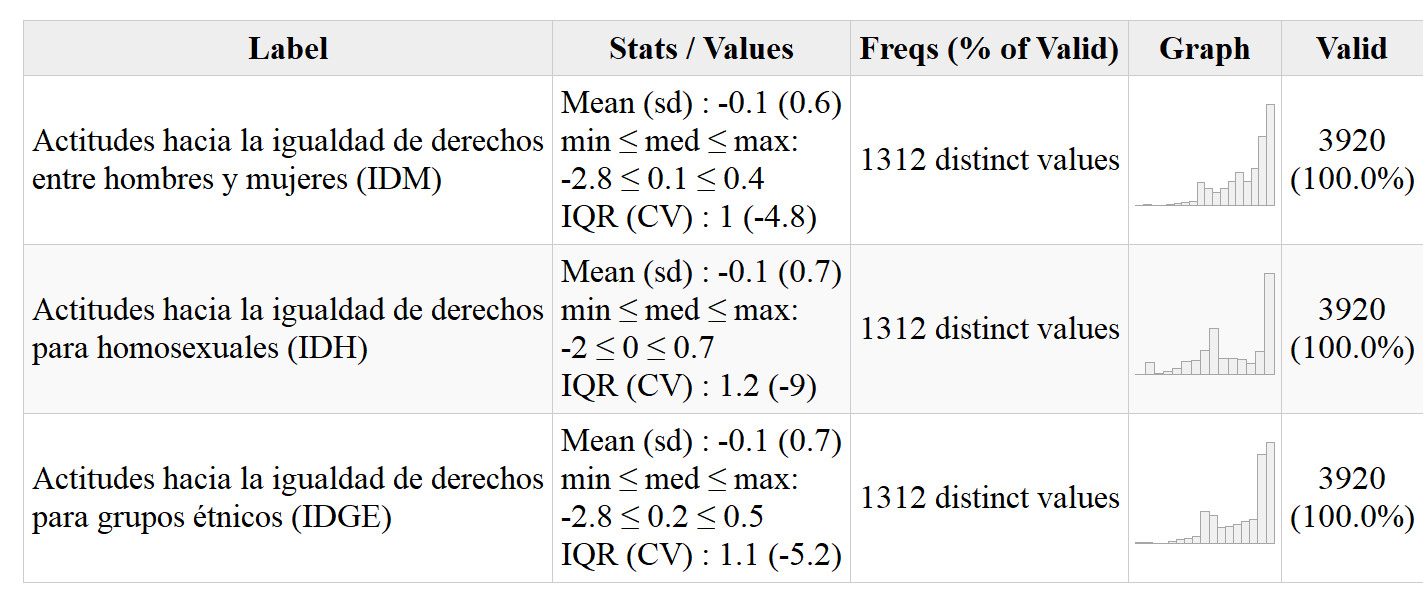
\includegraphics[width=\textwidth,height=0.5\textheight]{input/images/desc01_dep.png} \\
\bottomrule
\end{longtable}

En relación con la distribución de las variables independientes de nivel individual (que se presenta en la Tabla 4.2), cabe destacar que un 49.6\% de los estudiantes son de sexo masculino y un 50.4\% de sexo femenino, un 1.8\% de los estudiantes posee antecedentes migratorios y un 8.1\% de los estudiantes pertenece a un grupo étnico. El nivel de conocimiento cívico en la muestra varía entre 232.1 y 782.7 puntos, con una mediana de 503 puntos (media=498.6, ds=93.4). Por último, vale precisar también cómo se distribuyen los recursos socioeconómicos de la familia en la muestra analizada en este estudio. En relación con el nivel educacional de los padres, el 2.5\% no completo la enseñanza básica; el 9.8\% curso enseñanza básica; el 37.9\% completo la enseñanza media; el 19.6\% posee una carrera profesional o técnica; y el 30.3\% tiene una carrera universitaria o estudios de posgrado (magister o doctorado). En cuanto al estatus ocupacional de los padres, los valores varían entre 10 y 89, con una mediana de 42 puntos (media=46; ds=17.5). Finalmente, en lo que refiere a la cantidad de libros en el hogar, un 20.7\% posee entre 0 y 10 libros; un 30.1\% posee entre 11 y 25 libros; un 32.1\% posee entre 26 y 100 libros; un 9.7\% posee entre 101 y 200 libros; y un 7.4\% posee más de 200 libros.

\begin{longtable}[]{@{}l@{}}
\caption{\label{tab:unnamed-chunk-7}Variables independientes nivel individual}\tabularnewline
\toprule
\endhead
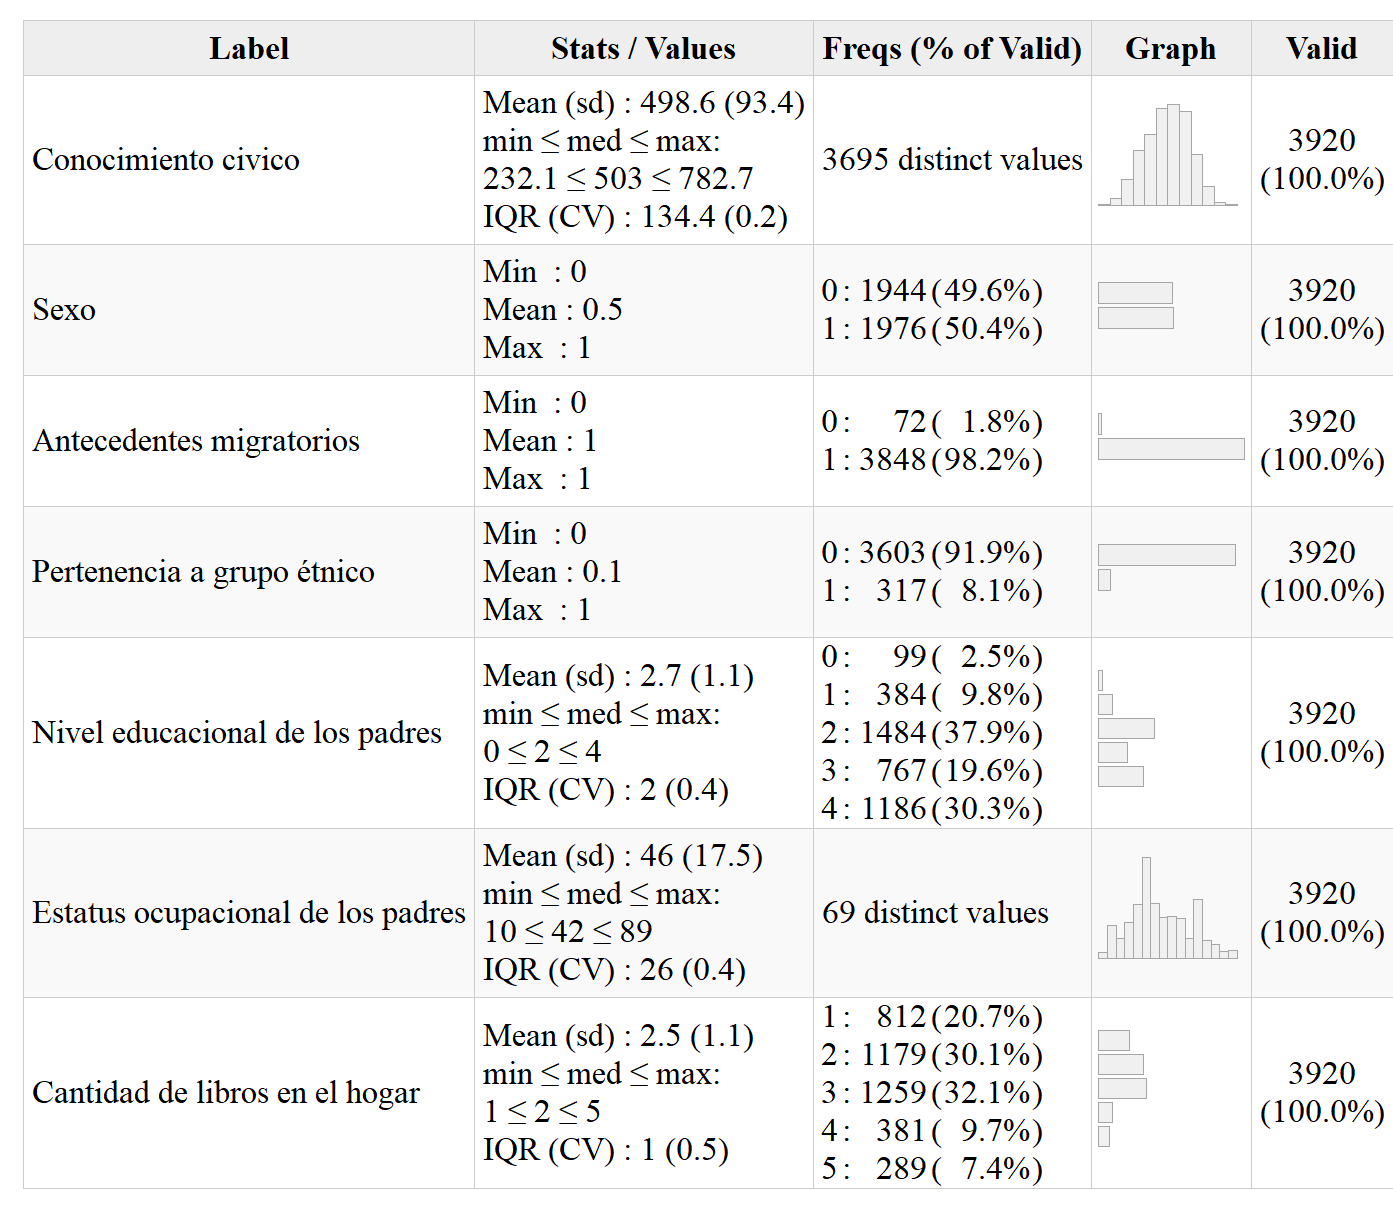
\includegraphics[width=\textwidth,height=0.5\textheight]{input/images/desc01_indep_ind.png} \\
\bottomrule
\end{longtable}

Por otro lado, en la Tabla 4.3 se presenta la distribución de las variables relativas a las características y prácticas de la escuela. La proporción de niñas en el aula varía entre 0 y 1 (media=0.5, ds=0.2), teniendo una distribución muy similar a la normal. La proporción de estudiantes pertenecientes a un grupo étnico varía entre 0 y 0.6 (media=0.1, ds=0.1), concentrándose la mayoría de las aulas en los valores más bajos (es decir, la mayoría tiene una baja proporción de estudiantes pertenecientes a grupos étnicos). La proporción de estudiantes con antecedentes migratorios varía entre 0 y 0.4 (media=0, ds=0), lo que indica que la gran mayoría de las escuelas tiene una muy baja proporción de estudiantes con antecedentes migratorios. En relación con la apertura a la discusión en el aula, calculada a partir de puntuaciones factoriales, varía entre -1 y 0.6, y tanto su media como su mediana es 0 (ds=0.3). Las tres variables relativas al clima escolar también han sido calculadas a partir de puntuaciones factoriales, distribuyéndose del siguiente modo: (1) las relaciones entre estudiantes y profesores varían entre -1.1 y 0.7 (ds=0.3), (2) las relaciones entre estudiantes varían entre -0.9 y 0.9 (ds=0.3), y (3) las situaciones de violencia física, emocional o verbal varían entre -1.2 y 1.5 (ds=0.6) (además, vale precisar que las tres variables tienen una media y una mediana igual a 0).

\begin{longtable}[]{@{}l@{}}
\caption{\label{tab:unnamed-chunk-8}Variables independientes nivel escuela}\tabularnewline
\toprule
\endhead
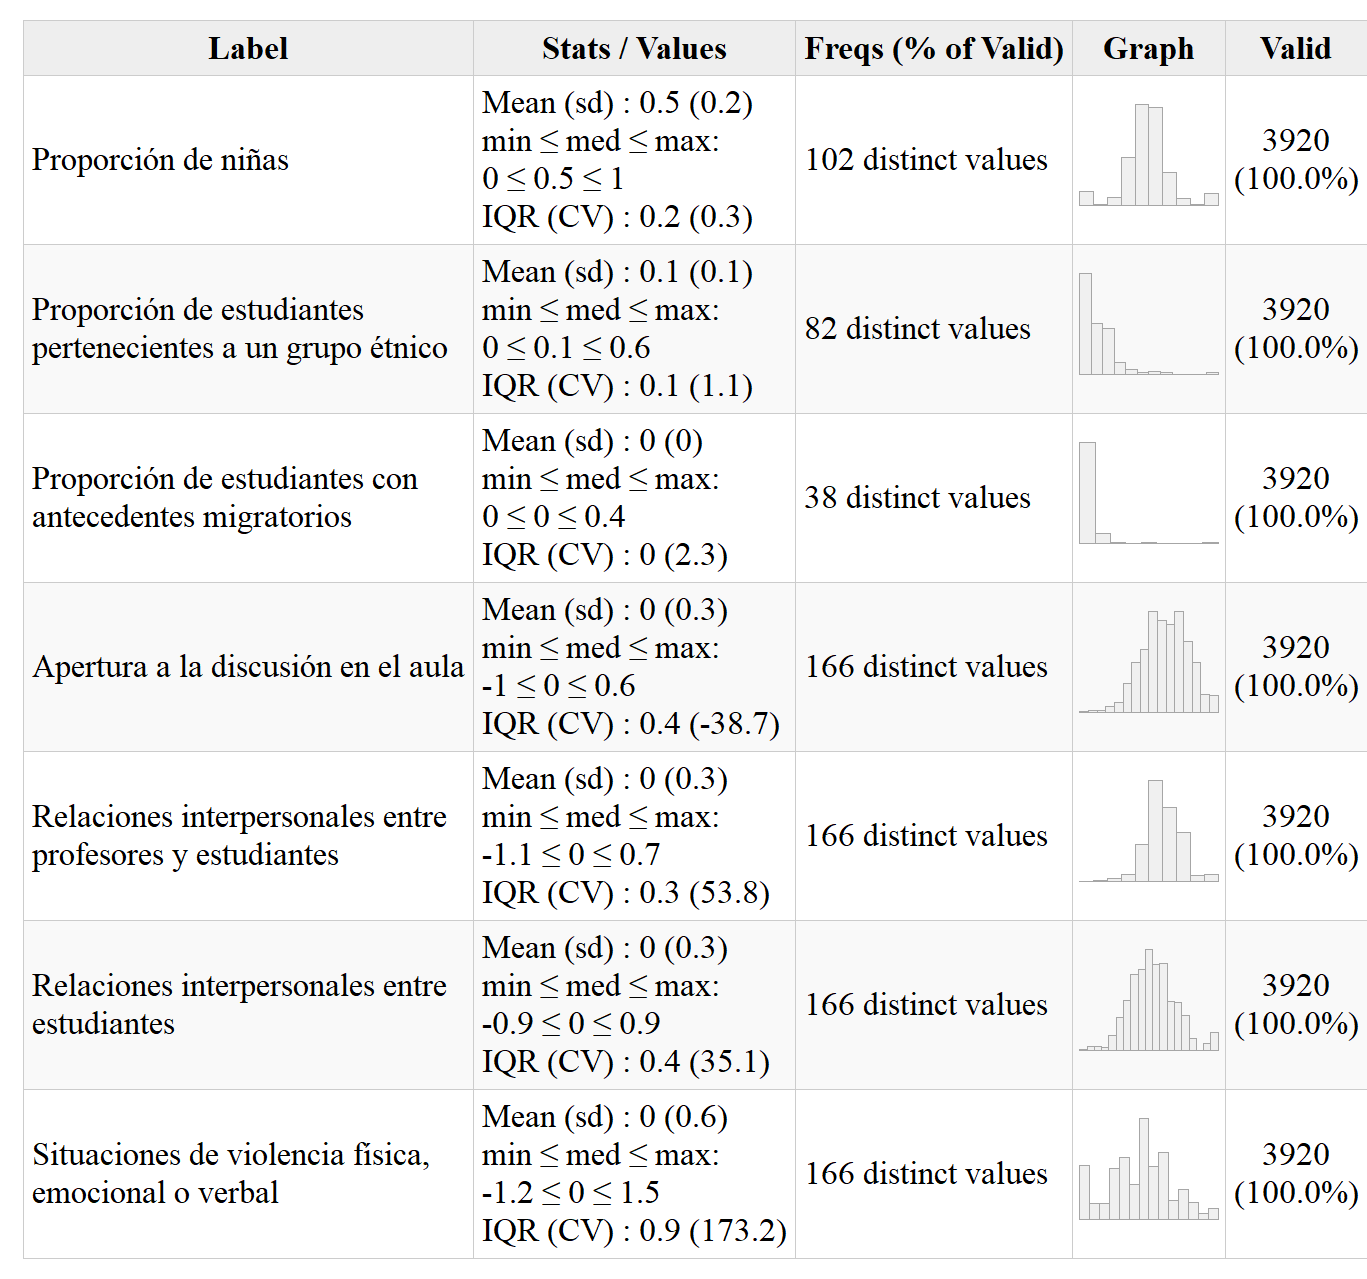
\includegraphics[width=\textwidth,height=0.5\textheight]{input/images/desc01_indep_col.png} \\
\bottomrule
\end{longtable}

\hypertarget{anuxe1lisis-multinivel}{%
\section{Análisis multinivel}\label{anuxe1lisis-multinivel}}

En esta sección se analizan los efectos tanto de las características individuales como de las características y prácticas de la escuela en tres dimensiones de las actitudes hacia la igualdad de derechos. Los resultados de los modelos de regresión multinivel se presentan primero en una tabla y después en un gráfico con los coeficientes beta estandarizados.

Antes de presentar los resultados de los modelos estimados, cabe precisar la correlación intraclase de cada variable dependiente. Este coeficiente representa el porcentaje de variación entre escuelas de la varianza de cada variable dependiente. Para la dimensión de actitudes hacia la igualdad de derechos entre hombres y mujeres la correlación intraclase corresponde a un 9.72\% de la varianza de las actitudes de los estudiantes. Para la dimensión de actitudes hacia la igualdad de derechos para grupos étnicos la correlación intraclase es un 9.48\% de la varianza de estas actitudes. Por último, para la dimensión de actitudes hacia la igualdad de derechos para homosexuales la correlación intraclase corresponde a un 7.57\% de la varianza de estas actitudes.

En la siguiente tabla se presentan los resultados de los modelos de regresión donde se estiman los efectos directos de las variables independientes en las tres variables dependientes. En el listado de predictores (o variables independientes) se presentan primero las variables individuales que caracterizan a los estudiantes y después variables del contexto, como la caracterización del curso en términos de composición y la apertura a la discusión.

\begin{longtable}[]{@{}l@{}}
\caption{\label{tab:unnamed-chunk-9}Modelo teórico}\tabularnewline
\toprule
\endhead
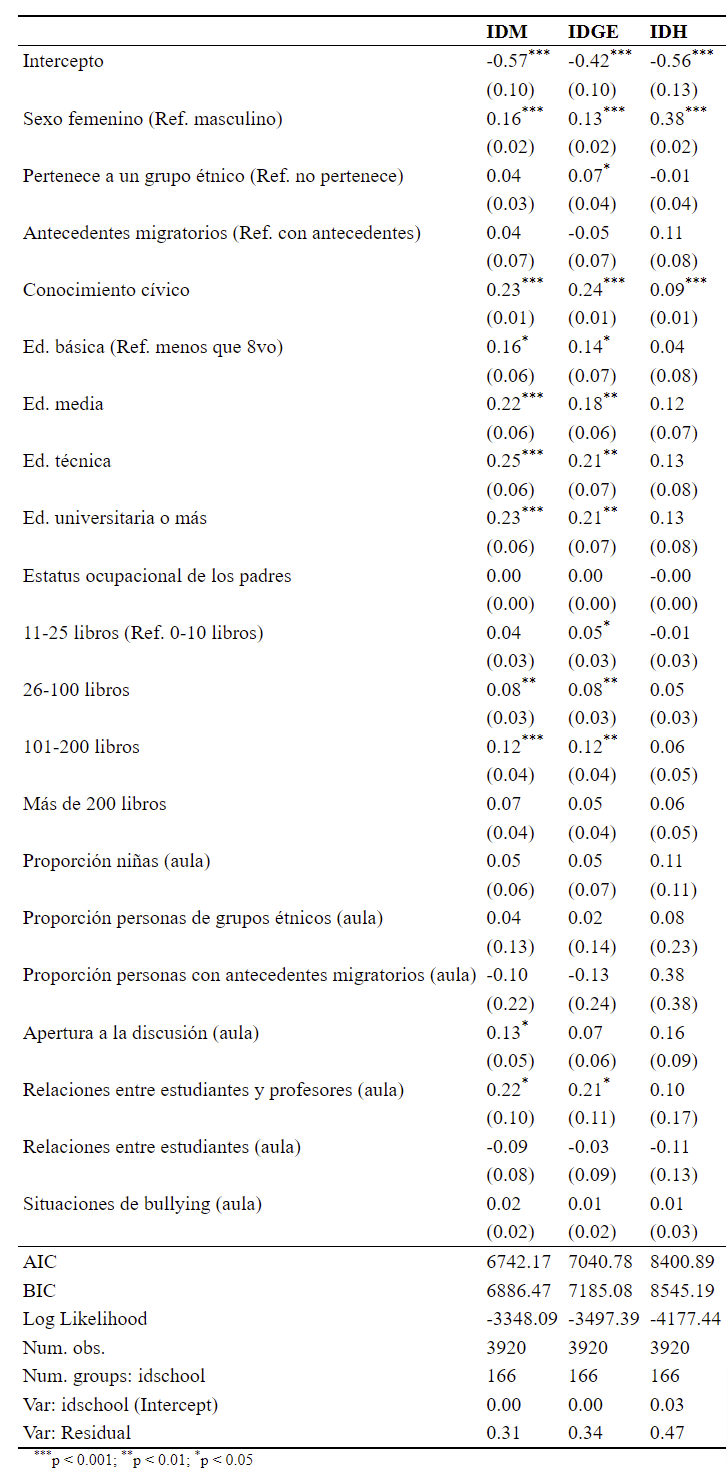
\includegraphics[width=\textwidth,height=0.9\textheight]{input/images/app_mod.png} \\
\bottomrule
\end{longtable}

Respecto a las características individuales, se evidencia que pertenecer al sexo femenino y que el nivel conocimiento cívico del estudiante se asocian positiva, significativa y consistentemente con las tres dimensiones analizadas de las actitudes hacia la igualdad de derechos. El efecto del sexo es especialmente fuerte en lo que refiere a las actitudes hacia la igualdad de derechos para homosexuales, mientras que el efecto del conocimiento cívico es particularmente bajo en dicha dimensión. Los efectos de estas variables en las otras dos dimensiones son muy similares entre sí. Por su parte, el análisis diferenciado de los efectos de los tres tipos de recursos socioeconómicos permite precisar que el nivel educacional de los padres y la cantidad de libros en el hogar tienen un efecto significativo en las actitudes hacia la igualdad de derechos entre hombres y mujeres, y para los grupos étnicos, pero prácticamente no influyen en las actitudes hacia la igualdad de derechos para los homosexuales. Contrariamente a lo hipotetizado, la ocupación de los padres, el origen étnico y los antecedentes migratorios no poseen efectos significativos. Los modelos explican el 13.49\%, el 7.1\% y el 10\% de la varianza entre individuos respectivamente, siguiendo el cálculo de R2 B\&R.

Respecto a las características de la escuela, los resultados indican que sólo las buenas relaciones entre estudiantes y profesores fomentan una actitud más favorable a la igualdad de derechos entre hombres y mujeres y para grupos étnicos, aunque no las fomenta en lo que refiere a los homosexuales. La apertura a la discusión en el aula posee un efecto positivo sobre la actitud hacia la igualdad de derechos para mujeres, pero no se ha encontrado evidencia que respalde esta relación en lo que refiere a las actitudes hacia la igualdad de derechos para grupos étnicos y homosexuales. Por último, la composición del curso en términos de género, pertenencia a grupos étnicos y antecedentes migratorios parece no afectar las actitudes de los estudiantes. Los modelos son ampliamente capaces de explicar las diferencias entre escuelas, los dos primeros explican más del 96\% de la varianza a nivel dos, mientras que el tercero explica un cuarto. Sin embargo, cabe precisar que estos resultados se deben analizar con cautela, ya que es probable que estos efectos estén sobredimensionados por la cantidad de variables predictoras a nivel 2 en contraste con la poca varianza en este nivel.

El siguiente gráfico nos muestra los efectos estandarizados, lo que nos permite comparar la magnitud del efecto de las distintas variables. Podemos apreciar que las variables que tienen un impacto más relevante son individuales, más específicamente, la pertenencia al sexo femenino, el conocimiento cívico y el nivel educativo de los padres (aunque está última no tiene un efecto consistente en las actitudes hacia la igualdad de derechos para homosexuales, de hecho sólo el nivel educativo más alto tiene un efecto significativo en esta variable). Por su parte, las variables del aula no logran generar cambios mayores a 0.25 desviaciones estándar, siendo las buenas relaciones entre estudiantes y profesores la variable con un tamaño de efecto más grande (aunque este efecto no es significativo en la dimensión que refiere a los homosexuales).

\begin{figure}[H]

{\centering 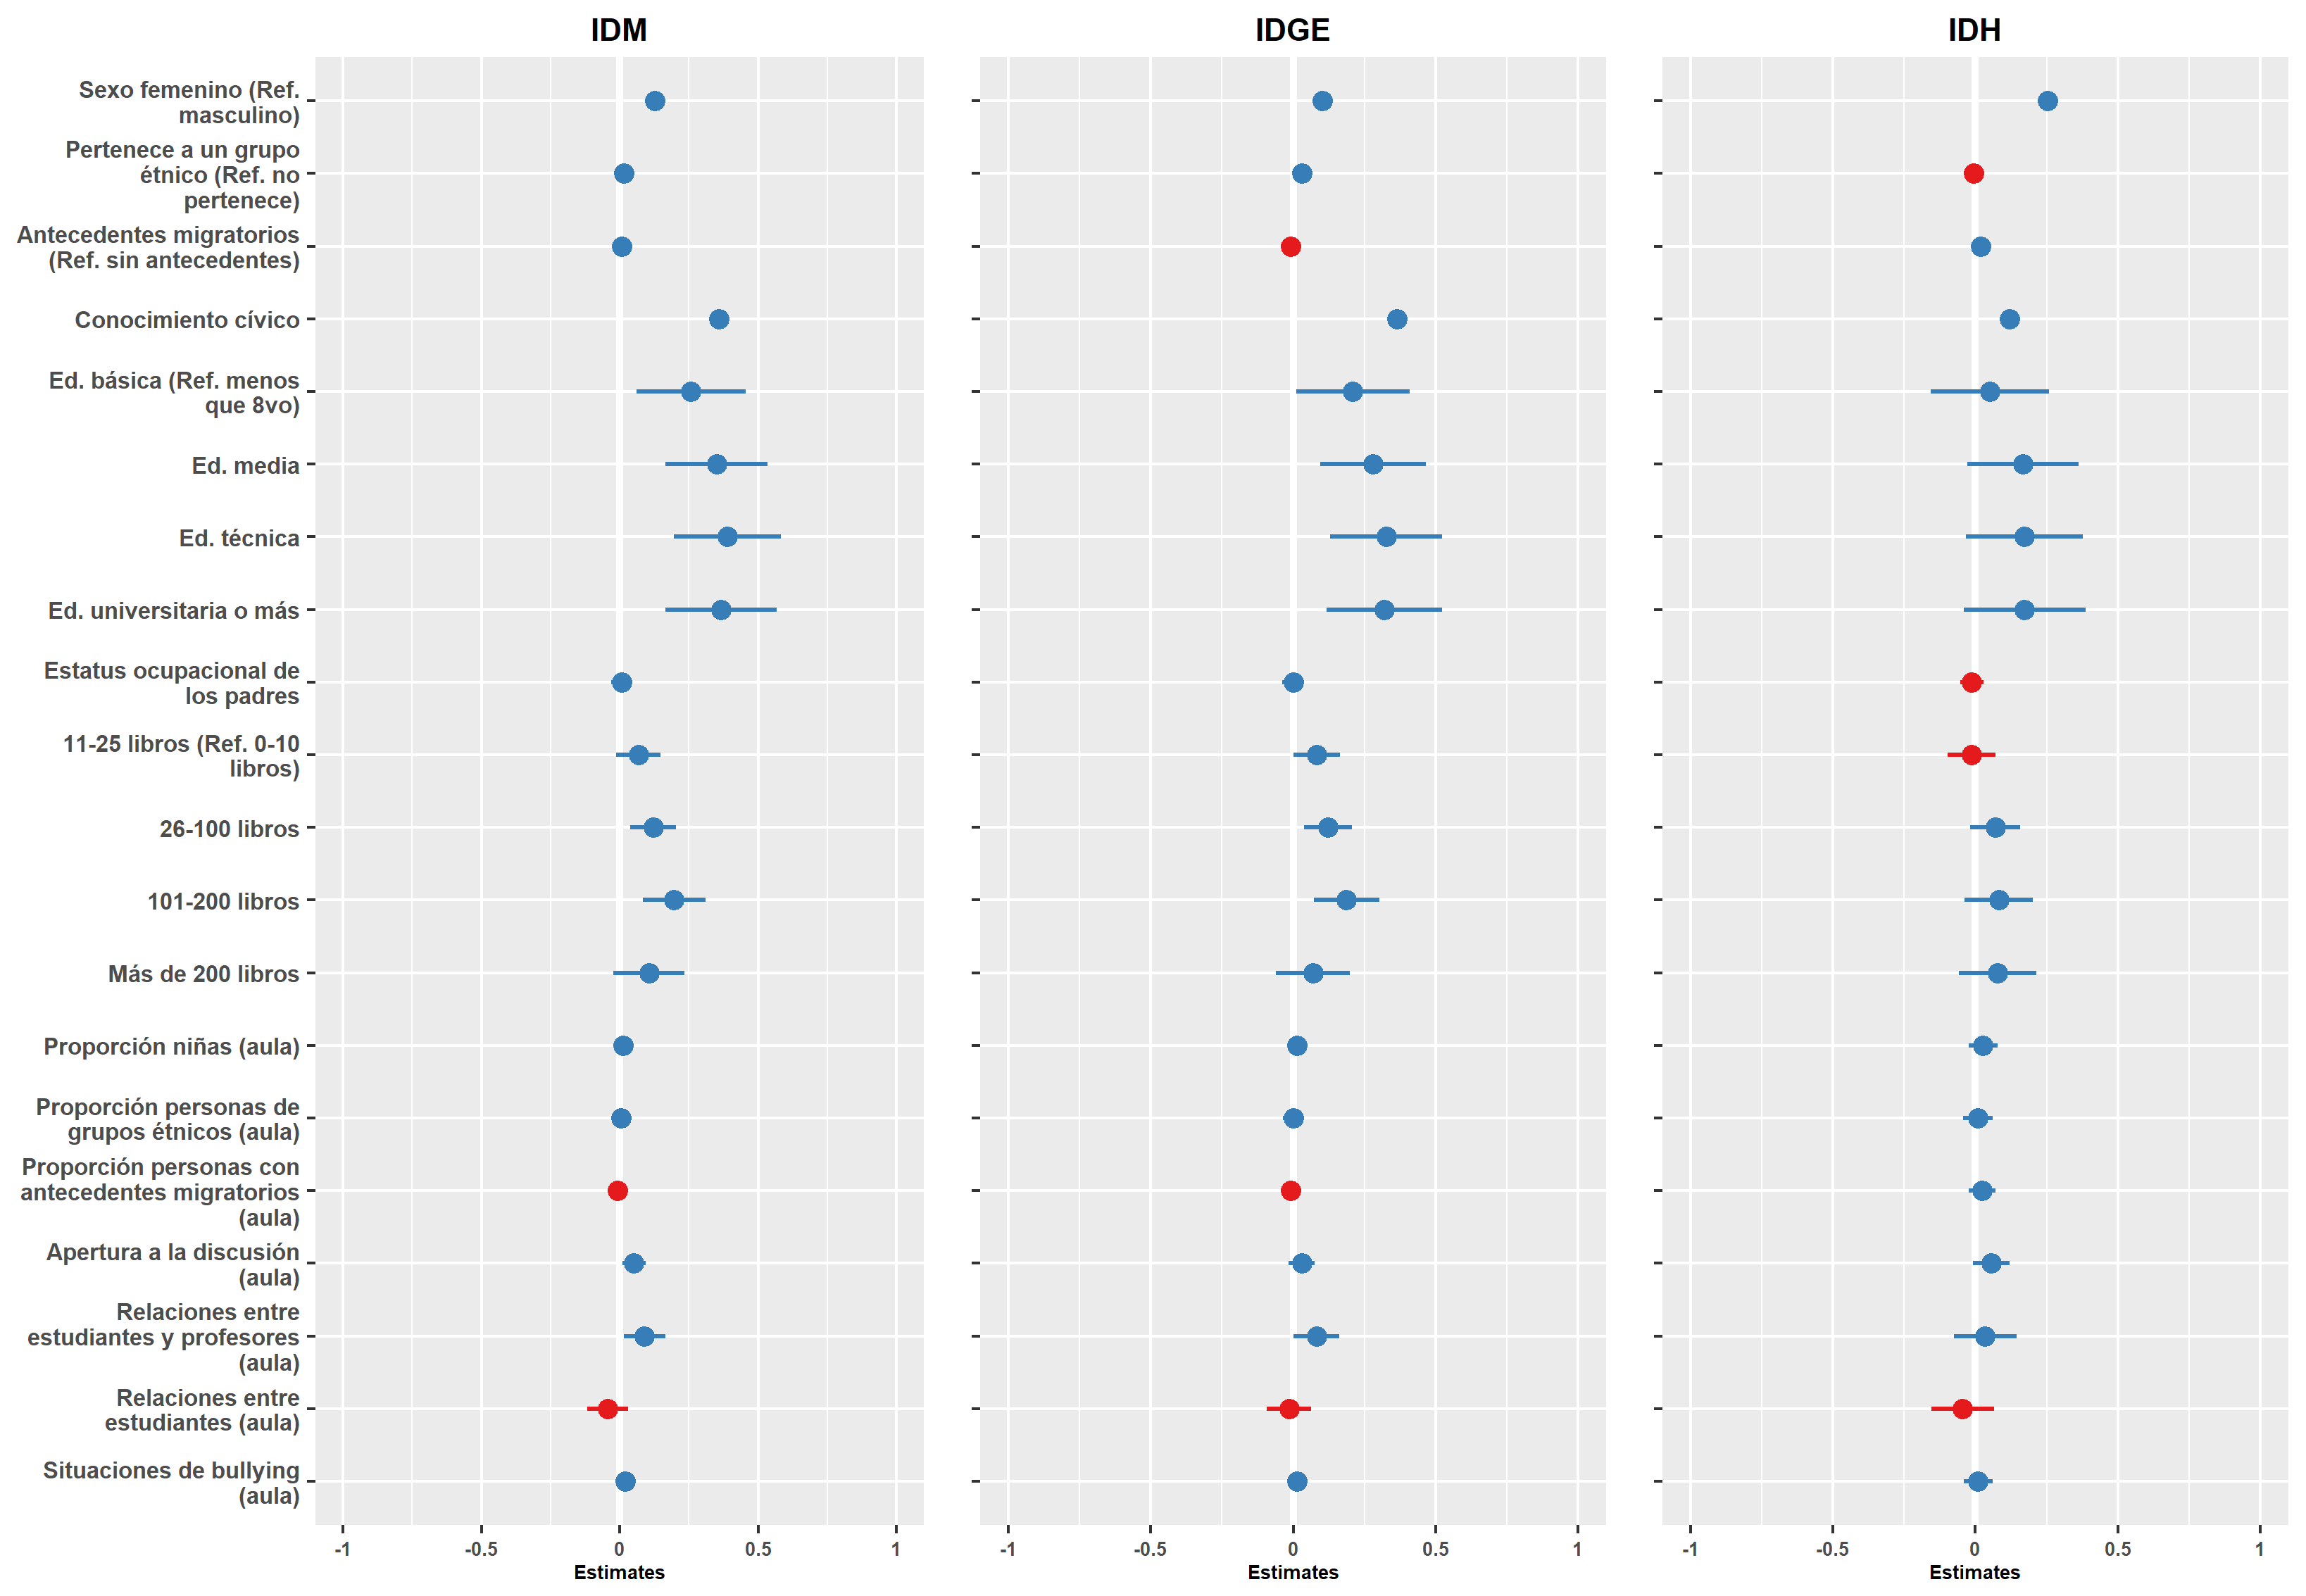
\includegraphics[width=0.9\linewidth]{input/images/EFECTOSTABLAREGRESION} 

}

\caption{Gráfico Modelos Multinivel}\label{fig:unnamed-chunk-10}
\end{figure}

\newpage

\hypertarget{efectos-de-interacciuxf3n}{%
\subsection{Efectos de interacción}\label{efectos-de-interacciuxf3n}}

Para indagar en el objetivo general de esta investigación se requiere hacer un análisis de los posibles efectos de interacción entre las variables de nivel individual y las variables de nivel escuela, con el propósito de dimensionar en qué medida características y prácticas de las escuelas tienen (o no) la capacidad de afectar la relación entre las actitudes hacia la igualdad de derechos del estudiante y sus características individuales. Para ello, antes de testear las hipótesis de interacción se estimaron modelos de regresión multinivel para cada variable dependiente, aleatorizando la pendiente de las distintas variables independientes de nivel individual. En otras palabras, con el objetivo de evaluar si los efectos de las variables independientes de nivel individual varían entre escuelas, se estimaron distintos modelos para cada variable dependiente. En cada uno de estos se especificaba la aleatorización de una de las variables independientes de nivel individual para una de las variables dependientes, proceso que se repitió sucesivamente hasta analizar la relación con todas las características individuales incorporadas en el estudio.

Este análisis permitió concluir que, tanto para las actitudes hacia la igualdad de derechos entre hombres y mujeres como para las actitudes hacia la igualdad de derechos para grupos étnicos, el efecto del sexo y del nivel de conocimiento cívico varía entre escuelas, haciéndose posible proceder con los análisis de los efectos de interacción para estas dos variables dependientes. Sin embargo, en lo que refiere a las actitudes hacia la igualdad de derechos para homosexuales, ninguno de los efectos de las variables independientes de nivel individual varía entre escuelas, por lo que no fue posible proseguir con los análisis de interacción para esta variable dependiente.

Por consiguiente, esta sección se enfoca en indagar cuál/es características y prácticas de las escuelas tiene/n la capacidad de afectar la relación entre el sexo y las actitudes hacia la igualdad de derechos para mujeres y para grupos étnicos, así como también se indaga en las variables de nivel escuela que son capaces de afectar la relación entre el nivel de conocimiento cívico del estudiante y sus actitudes hacia la igualdad de derechos para los dos grupos precisados.

Se ha decidido evaluar la capacidad de moderación de la variable ``relación entre estudiantes y profesores'' dado que ha sido la única variable contextual que evidenció un efecto consistente (es decir, que afecta en ambas dimensiones y no sólo en una). En particular, evaluaremos la capacidad de esta variable para disminuir las diferencias en las actitudes hacia la igualdad de derechos para mujeres y grupos étnicos asociadas a las características individuales: sexo y nivel de conocimiento cívico.

Esta sección tiene dos grandes secciones, una para cada variable dependiente. Primero se evalúan modelos para predecir las actitudes hacia la igualdad de derechos entre hombres y mujeres, y luego la segunda sección enfoca en las actitudes hacia la igualdad de derechos para grupos étnicos. Además, cada una de estas secciones poseen a su vez dos subsecciones, una para evaluar la capacidad de las relaciones entre estudiantes y profesos para moderar el efecto del sexo y otra subsección donde se evalúa la capacidad de dicha variable para moderar el efecto del conocimiento cívico. En suma, este apartado cuenta con 4 subsecciones que mantienen la variable moderadora de nivel 2 (relación con los profesores) y cambian tanto la variable dependiente (actitudes hacia la igualdad de derechos para mujeres por un lado y para grupos étnicos por otro) como la variable independiente de nivel individual (sexo o conocimiento cívico del estudiante). En cada uno de estos subapartados se presentan los resultados de tres modelos: (1) el modelo multinivel para esa variable dependiente presentado en la Tabla 4.4 (por lo que incorpora el control estadístico de todas las variables independientes presentes en el modelo), (2) el modelo con pendiente aleatoria (se aleatoriza el efecto del sexo o del nivel de conocimiento cívico, según corresponda) y (3) el modelo con pendiente aleatoria e interacción entre niveles.

\hypertarget{las-buenas-relaciones-entre-estudiantes-y-profesores-como-factor-contextual-para-disminuir-las-diferencias-en-las-actitudes-hacia-la-igualdad-de-derechos-entre-hombres-y-mujeres.}{%
\subsubsection{Las buenas relaciones entre estudiantes y profesores como factor contextual para disminuir las diferencias en las actitudes hacia la igualdad de derechos entre hombres y mujeres.}\label{las-buenas-relaciones-entre-estudiantes-y-profesores-como-factor-contextual-para-disminuir-las-diferencias-en-las-actitudes-hacia-la-igualdad-de-derechos-entre-hombres-y-mujeres.}}

\hypertarget{moderando-el-efecto-del-sexo}{%
\paragraph{Moderando el efecto del sexo}\label{moderando-el-efecto-del-sexo}}

En la siguiente tabla se puede apreciar como las buenas relaciones con los docentes modera la relación entre el sexo del estudiante y sus actitudes hacia la igualdad de derechos para mujeres.

La tabla nos presenta cuatro parámetros especialmente relevantes: el intercepto, el efecto directo del sexo, el efecto directo de las buenas relaciones con los profesores y el efecto de moderación. Además, incluye distintas estimaciones de ajuste, presentándose los R2 a nivel uno (individual) y nivel dos (escuela), y los R2 sin y con los efectos aleatorios. Además, se presenta la significación de un anova que nos indica si el modelo es significativamente distinto al anterior. Como se enunció en el párrafo anterior, todos los modelos están controlados por las demás variables, pero se han omitido los coeficientes para simplificar la presentación de los resultados.

\begin{longtable}[]{@{}l@{}}
\caption{\label{tab:unnamed-chunk-11}Efectos de interacción entre el sexo y las relaciones con los profesores, en las actitudes hacia la igualdad de derechos para mujeres}\tabularnewline
\toprule
\endhead
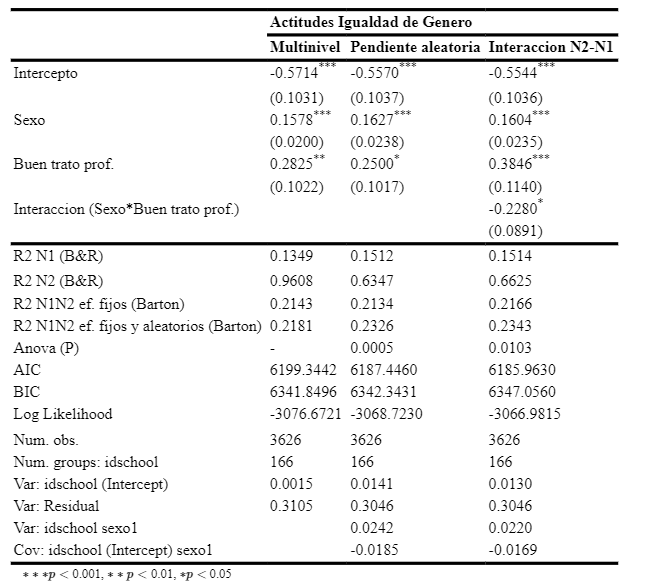
\includegraphics[width=\textwidth,height=0.8\textheight]{input/images/INTERACCION1.png} \\
\bottomrule
\end{longtable}

Como pudimos ver en la sección de análisis multinivel, el ser mujer se asocia positivamente con tener actitudes favorables a la igualdad de derechos entre hombres y mujeres, lo cual podemos observar en el modelo ``Multinivel''. En estas actitudes las niñas tienen en promedio 0.15 desviaciones estándar más que los hombres. De modo similar, cuando las relaciones con los profesores aumentan en una desviación estándar, las actitudes de los jóvenes hacia la igualdad de derechos para mujeres aumenta en promedio 0.28 desviaciones estándar.

Si incorporamos al modelo la posibilidad de que el efecto del sexo sobre estas actitudes varíe entre escuelas, se obtiene un modelo con mejor R2 general (Cuarto R2 en la tabla). Además, la prueba de anova que compara el modelo con y sin pendientes aleatorias nos indica que ambos modelos son significativamente distintos, siendo el modelo con pendientes aleatorias significativamente mejor.

El modelo de interacción incorpora un nuevo parámetro. Este nos indica cuánto disminuye el efecto de ser mujer cuando se está en un curso con buenas relaciones con los profesores, siendo posible afirmar que en la medida en que las relaciones con el profesor aumentan en una desviación estándar, el efecto de la variable sexo en las actitudes hacia la igualdad de derechos para mujeres disminuye en promedio 0.22 puntos. Esta interacción es significativa con un 95\% de confianza. El modelo posee una capacidad explicativa ligeramente mejor que el modelo con pendiente aleatoria, pero cabe destacar que los resultados de la prueba anova indican que esta pequeña diferencia mejora significativamente el modelo, con un 95\% de confianza.

Para comprender mejor esta interacción se presenta a modo ilustrativo el siguiente gráfico. Este nos permite comprender cardinalmente el efecto de la interacción (aunque no es la representación más adecuada para dimensionar su efecto, ya que se exponen predicciones con los casos extremos).

Lo interesante de este gráfico es que nos permite observar como las diferencias en actitudes a la igualdad de derechos entre hombres y mujeres disminuye cuando existe una excelente relación con los profesores. Aunque en mujeres no es tan notoria la diferencia entre tener o no una buena relación con los profesores, entre los hombres este factor genera más efecto, permitiendo (en los casos con la mayor puntuación de buenas relaciones con los profesores) que los niños alcancen los mismos niveles que las niñas en este tipo de actitudes.

\begin{figure}[H]

{\centering 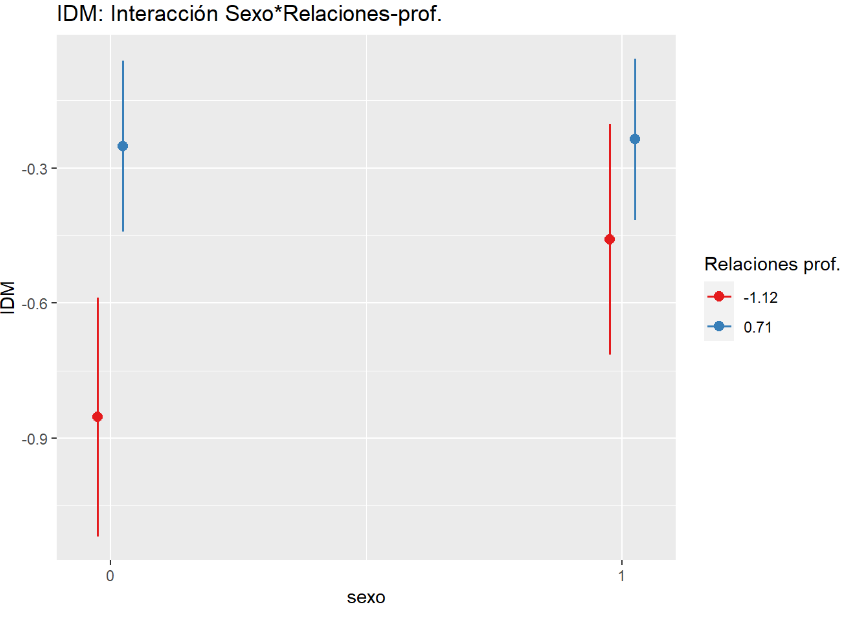
\includegraphics[width=0.9\linewidth]{input/images/PLOTINT1} 

}

\caption{Grafico de interacción entre el sexo y las relaciones con los profesores, en las actitudes hacia la igualdad de derechos para mujeres}\label{fig:unnamed-chunk-12}
\end{figure}

\newpage

\hypertarget{moderando-el-efecto-del-conocimiento-cuxedvico}{%
\paragraph{Moderando el efecto del conocimiento cívico}\label{moderando-el-efecto-del-conocimiento-cuxedvico}}

En esta subsección se evalúa la capacidad de las buenas relaciones con los profesores para disminuir el efecto del conocimiento cívico sobre las actitudes hacia la igualdad de derechos para las mujeres.

Tanto cuando se incorpora la pendiente aleatoria como cuando se precisa la interacción se obtienen mejoras en la capacidad explicativa de los modelos. Respecto a los tamaños de los efectos, se observa que al incorporar la pendiente aleatoria el modelo mejora en un 0,8\% la varianza explicada, mientras que al comparar el modelo inicial y el modelo con interacción se logra una mejora del 1,2\%. Cabe destacar que ambas mejoras son significativas al comparar los modelos.

El efecto de la interacción nos indica que cuando existen buenas relaciones con los profesores (o más precisamente, cuando las relaciones con los profesores aumentan en una desviación estándar) el efecto del conocimiento sobre las actitudes hacia la igualdad de derechos para mujeres (que es 0.2226) disminuye en -0.1662 unidades. En otras palabras, si un estudiante posee un bajo conocimiento cívico, esto afectará menos sus actitudes hacia la igualdad de derechos entre hombres y mujeres si asiste a un aula donde hay una buena relación con los profesores.

\begin{longtable}[]{@{}l@{}}
\caption{\label{tab:unnamed-chunk-13}Efectos de interacción entre el nivel de conocimiento cívico y las relaciones con los profesores, en las actitudes hacia la igualdad de derechos para mujeres}\tabularnewline
\toprule
\endhead
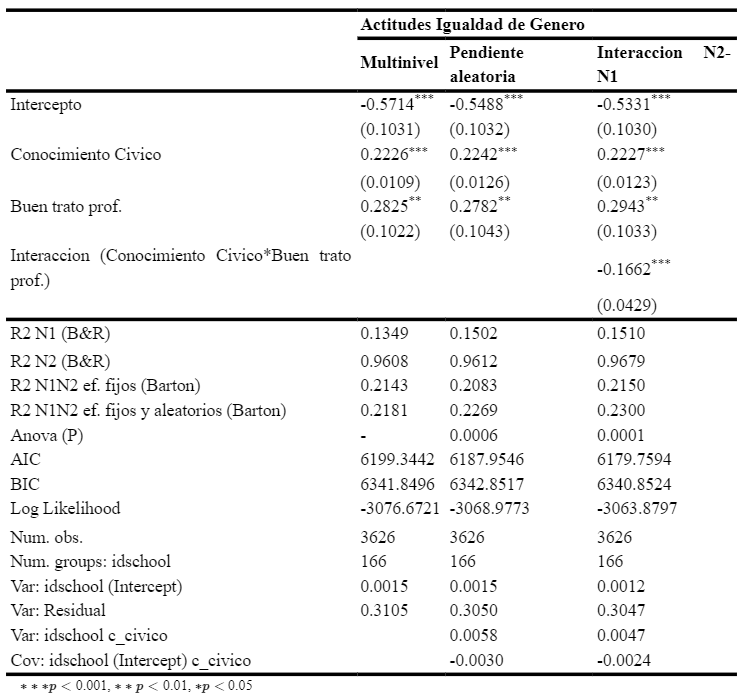
\includegraphics[width=\textwidth,height=0.8\textheight]{input/images/INTERACCION2.png} \\
\bottomrule
\end{longtable}

El siguiente gráfico nos muestra como la pendiente (es decir, el efecto) del conocimiento cívico es mucho menos pronunciada en un contexto que posee una buena relación con sus docentes.

\begin{figure}[H]

{\centering 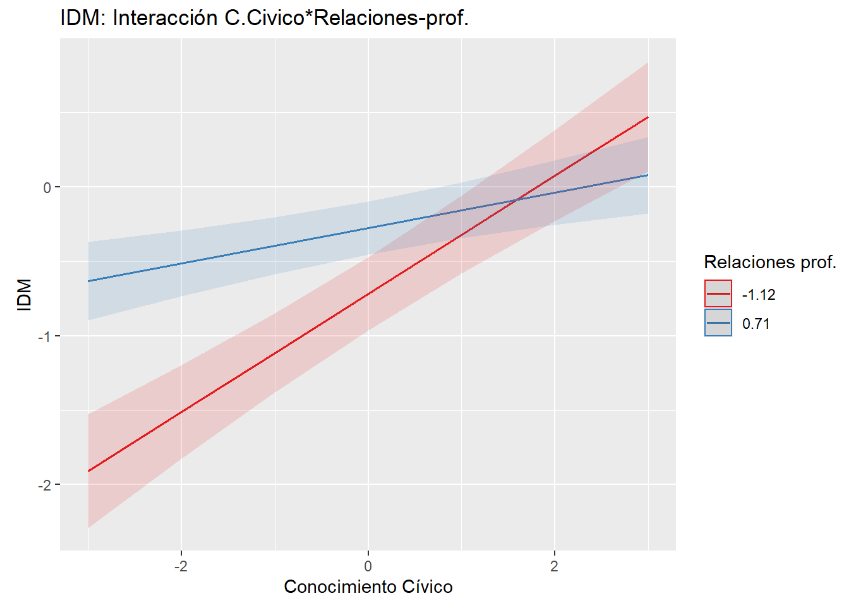
\includegraphics[width=0.9\linewidth]{input/images/PLOTINT2} 

}

\caption{Grafico de interacción entre el conocimiento cívico y las relaciones con los profesores, en las actitudes hacia la igualdad de derechos para mujeres}\label{fig:unnamed-chunk-14}
\end{figure}

\hypertarget{las-buenas-relaciones-entre-estudiantes-y-profesores-como-factor-contextual-para-disminuir-las-diferencias-en-las-actitudes-hacia-la-igualdad-de-derechos-para-grupos-uxe9tnicos.}{%
\subsubsection{Las buenas relaciones entre estudiantes y profesores como factor contextual para disminuir las diferencias en las actitudes hacia la igualdad de derechos para grupos étnicos.}\label{las-buenas-relaciones-entre-estudiantes-y-profesores-como-factor-contextual-para-disminuir-las-diferencias-en-las-actitudes-hacia-la-igualdad-de-derechos-para-grupos-uxe9tnicos.}}

En esta sección se analiza la capacidad de las buenas relaciones con los profesores para moderar el efecto del sexo y el conocimiento cívico en las actitudes hacia la igualdad de derechos para grupos étnicos.

A modo de resumen, se da cuenta de cómo esta cualidad del aula puede moderar el efecto del conocimiento cívico, pero no el del sexo.

En la siguiente tabla se observan los modelos para indagar en el efecto de interacción. Se evalúa la capacidad de las relaciones con el profesor de moderar el efecto del sexo en las actitudes a la igualdad de derechos para grupos étnicos.

Como se puede observar el efecto de la interacción no es significativo, lo cual se condice con que la mejora de la capacidad explicativa del modelo con la interacción tampoco lo es.

Por ello no se indagará más en este punto. No obstante, cabe destacar que, si existe variabilidad en la pendiente de la relación entre distintos contextos, por lo que cabe preguntarse qué características o prácticas de la escuela podrían explicar esta variación.

\begin{longtable}[]{@{}l@{}}
\caption{\label{tab:unnamed-chunk-15}Efectos de interacción entre el sexo y las relaciones con los profesores, en las actitudes hacia la igualdad de derechos para grupos étnicos}\tabularnewline
\toprule
\endhead
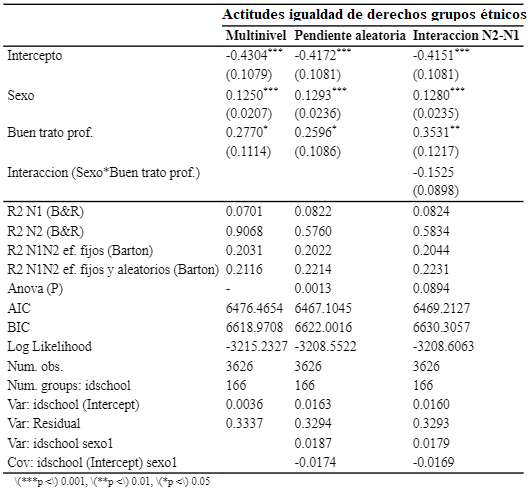
\includegraphics[width=\textwidth,height=0.8\textheight]{input/images/INTERACCION3.png} \\
\bottomrule
\end{longtable}

\hypertarget{moderando-el-efecto-del-conocimiento-cuxedvico-1}{%
\paragraph{Moderando el efecto del conocimiento cívico}\label{moderando-el-efecto-del-conocimiento-cuxedvico-1}}

Esta tabla evalúa la capacidad de moderación que posee el buen trato de los profesores en el aula sobre el efecto del conocimiento cívico en las actitudes hacia la igualdad de derechos para grupos étnicos.

En la tabla se puede apreciar que son significativos los efectos tanto del conocimiento cívico como de las buenas relaciones con los profesores, efectos que se mantiene pese a la incorporación de nuevas especificaciones en el modelo.

El efecto de moderación es significativo, y por cada desviación estándar que aumenta las relaciones con los profesores, disminuye 0.13 el efecto del conocimiento cívico en las actitudes hacia la igualdad de derechos para grupos étnicos. El modelo con pendientes aleatorias y con interacción son significativamente mejores que los modelos anteriores.

La incorporación del parámetro de interacción mejora en un 0.67\% el R2 general del modelo. Asimismo, cabe destacar que incorporar estas variables mejora un 6\% el R2 nivel 2 y un 1.26\% el R2 nivel 1.

\begin{longtable}[]{@{}l@{}}
\caption{\label{tab:unnamed-chunk-16}Efectos de interacción entre el conocimiento cívico y las relaciones con los profesores, en las actitudes hacia la igualdad de derechos para grupos étnicos}\tabularnewline
\toprule
\endhead
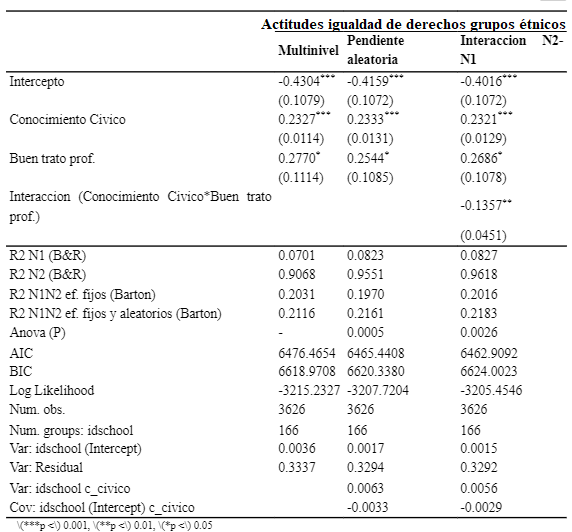
\includegraphics[width=\textwidth,height=0.8\textheight]{input/images/INTERACCION4.png} \\
\bottomrule
\end{longtable}

Para comprender la dirección de la interacción se presenta el siguiente gráfico, donde se puede apreciar una disminución de la pendiente cuando existe una mejor relación con los profesores.

\begin{figure}[H]

{\centering 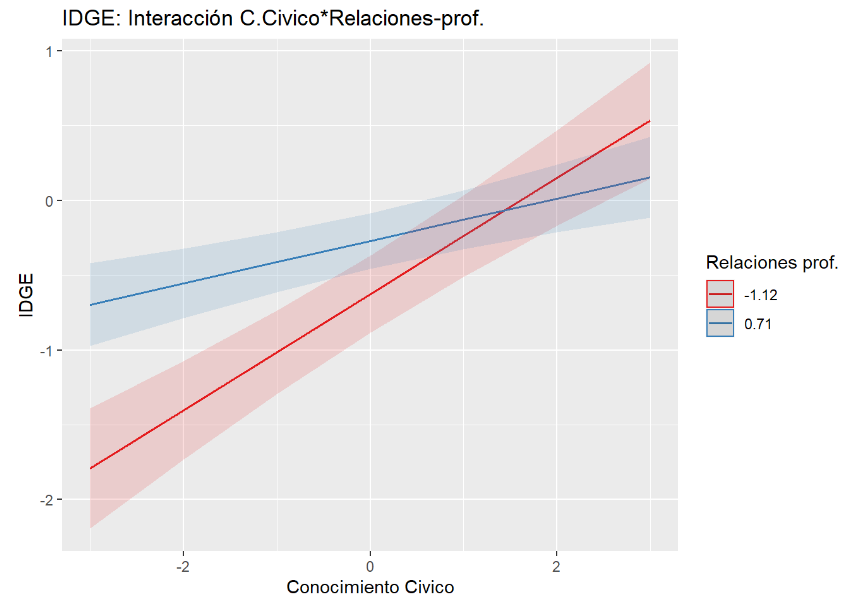
\includegraphics[width=0.9\linewidth]{input/images/PLOTINT4} 

}

\caption{Grafico interacción entre el conocimiento cívico y las relaciones con los profesores, en las actitudes hacia la igualdad de derechos para grupos étnicos}\label{fig:unnamed-chunk-17}
\end{figure}

\hypertarget{conclusiones}{%
\chapter{Conclusiones}\label{conclusiones}}

Esta tesis analizó, en población estudiantil, los factores asociados a las actitudes hacia la igualdad de derechos en tres dimensiones: entre hombres y mujeres, para grupos étnicos y para homosexuales. Desde la teoría de recursos y desde la hipótesis de las posiciones de desventaja, se esperaba que el poseer recursos socioeconómicos o culturales y el pertenecer a grupos en desventaja fomente una actitud positiva hacia la igualdad de derechos hacia distintos grupos. Asimismo, en base a estudios sobre formación ciudadana se esperaba que características y prácticas de la escuela, como las relaciones con los profesores y la composición de las aulas influyeran en las actitudes hacia la igualdad de derechos. Basándose en ambas líneas de investigación, esta tesis se propuso indagar en si características de la escuela, como espacio fundamental de socialización, pueden disminuir el efecto de las características individuales sobre las actitudes hacia igualdad de derechos. Dicho de otro modo, esta tesis propone que un clima escolar donde se dan buenas relaciones interpersonales entre los profesores y/o estudiantes puede hacer que estudiantes de sexo masculino o con bajos niveles de conocimiento cívico posean igualmente buenas actitudes hacia la igualdad de derechos.

En primer lugar, los resultados nos permiten comprobar parcialmente el efecto de las características individuales. A partir del modelo multinivel, se evidencia que los recursos socioeconómicos afectan parcialmente las actitudes a la igualdad de derechos. Ninguno de los recursos analizados afecta de forma relevante y consistente las actitudes hacia la igualdad de derechos para homosexuales. No obstante, tanto la cantidad de libros en el hogar como la educación de los padres se relacionan positivamente con las actitudes hacia la igualdad de derechos entre hombres y mujeres y para grupos étnicos. En relación con la hipótesis de la posición de desventaja, es posible afirmar que pertenecer al sexo femenino se asocia positivamente con las actitudes hacia la igualdad de derechos en las tres dimensiones en estudio (y especialmente en lo relativo a los homosexuales), mientras que los antecedentes migratorios no se relacionan significativamente con estas actitudes de los jóvenes y la pertenencia a un grupo étnico sólo afecta las actitudes hacia la igualdad de derechos para grupos étnicos. El conocimiento cívico demostró tener un considerable efecto sobre las actitudes hacia la igualdad de derechos.

En segundo lugar, los análisis nos entregan información sobre el efecto de las características y prácticas de la escuela. De modo contrario a lo hipotetizado, las características de composición del aula analizadas no poseen un efecto relevante para explicar las actitudes hacia la igualdad de derechos, así como la apertura a la discusión en el aula tampoco presenta un efecto consistente en estas actitudes, asociándose positivamente sólo a las actitudes hacia la igualdad de derechos entre hombres y mujeres. Asimismo, en relación con el clima en el aula, las dimensiones de ``relaciones interpersonales entre estudiantes'' y de ``situaciones de violencia en la escuela'' no afectan significativamente las actitudes de los jóvenes hacia la igualdad de derechos en los tres factores analizados. Sin embargo, acorde a lo esperado, se pudo evidenciar un efecto positivo de las relaciones interpersonales entre estudiantes y profesores en las actitudes hacia la igualdad de derechos para dos de las tres dimensiones analizadas. De modo que, si un profesor desarrolla buenas relaciones con sus estudiantes estos tendrán más probabilidades de poseer actitudes favorables hacia la igualdad de derechos entre hombres y mujeres y para grupos étnicos.

En tercer lugar, los resultados dan luces sobre la hipótesis central de la tesis, que proponía que prácticas de la escuela podrían moderar las diferencias en las actitudes sobre la igualdad de derechos producidas por características individuales. A partir de la interacción multinivel se puede evidenciar que mejores relaciones con los profesores disminuyen las diferencias basadas tanto en el sexo como en el desigual conocimiento cívico de los estudiantes en dos de las tres dimensiones analizadas. Más específicamente, las buenas relaciones con el profesor en el aula son capaces de moderar o disminuir las diferencias tanto en las actitudes hacia la igualdad de derechos entre hombres y mujeres como en las actitudes hacia la igualdad de derechos para grupos étnicos. Sin embargo, pese a encontrar estos efectos significativos, es importante señalar que incluir estos efectos de moderación en los modelos aumenta levemente la capacidad explicativa de los mismos. Es decir, aunque este rasgo de la escuela es capaz de moderar las diferencias individuales señaladas, esta moderación es más bien leve y por ello estas conclusiones deben ser tomadas con precaución.

\hypertarget{discusiuxf3n}{%
\section{Discusión}\label{discusiuxf3n}}

En términos teóricos, sobre el efecto de las características de las escuelas, esta investigación nos entrega información importante respecto a los efectos. Desde la teoría del contacto intergrupal destacada por Allport (1954) y la teoría del ``efecto de los compañeros'' (Bellei, 2013) se esperaba un efecto relevante por los factores de composición. Más específicamente se esperaba, basados en las investigaciones de Caro y Schulz (2012); y de Isaac, Moslawski y Van der Werdf (2012), que la mayor presencia en el aula de personas pertenecientes a grupos desventajados fomentara actitudes más favorables a la igualdad de derechos. No obstante, en el caso de este estudio no ha sido posible encontrar esta asociación al considerar además otros factores influyentes, como el clima escolar, la apertura a la discusión en el aula y características individuales. Una pregunta interesante para indagar en otros estudios puede relacionarse con por qué en este contexto no se encuentra la relación esperada. Una posibilidad por estudiar refiere a las relaciones entre los estudiantes en contextos con más variedad de composición dentro del aula.

Sin duda, la conclusión más relevante de esta investigación versa sobre el rol que cumple el clima escolar por sí mismo y moderando las diferencias entre estudiantes sobre dos dimensiones de las actitudes hacia la igualdad de derechos. Siguiendo la evidencia levantada por tanto por Caro y Schulz (2012), como por Schulz y Ainley (2018) se esperaba un relevante efecto del clima escolar en las actitudes hacia la igualdad de derechos. Basados en esta premisa, la presente investigación diferenció las relaciones con el profesor de las relaciones entre estudiantes. Al diferenciar los efectos del clima del aula en tres dimensiones se pudo observar que buena parte del efecto del clima del aula se debe en particular a la relación que poseen los estudiantes con los profesores. El rol del trato con los profesores en la formación de las actitudes a la igualdad de derechos puede comprenderse como un efecto de socialización donde prima el comportamiento de figuras referentes de autoridad, como los docentes, frente a la relación entre los estudiantes.

En términos de política pública esto releva la importancia de fomentar una formación integral de los profesores, preparándolos no solo para enseñar sus respectivas asignaturas sino, también, para dotarlos con herramientas socioemocionales para mantener un buen trato y buenas relaciones con los estudiantes. Esto es relevante ya que el ejemplo del profesor parece especialmente importante en la formación de actitudes hacia la igualdad de derechos.

La apertura a la discusión en el aula, destacada por Barber, Torney-Purta y Fennelly (2010) no presentó efectos significativos al ser controlada por las otras variables de nivel individual y escolar. Una posible razón para esto es que el efecto positivo de la discusión en el aula se deba en realidad al efecto positivo que tiene esta práctica en las relaciones entre estudiantes y profesores, por lo que no es posible visualizar el efecto de la apertura a la discusión en el aula cuando se controla por las relaciones interpersonales con los docentes. Sería interesante poder indagar en la posible relación de mediación entre estas variables en próximas investigaciones.

Finalmente, me gustaría destacar dos elementos. En primer lugar, considero fundamental relevar que, contrario a lo esperado, en consideración de los resultados de esta investigación es posible proponer que las actitudes hacia la igualdad de derechos para homosexuales siguen una dinámica relativamente distinta a las otras dos dimensiones de las actitudes hacia la igualdad de derechos. Entre las variables independientes analizadas, es una cantidad menor las que tienen un efecto significativo en este tipo de actitudes (en comparación a las otras dos dimensiones analizadas) y las pendientes de estos efectos no varían entre escuelas, por lo que no fue posible indagar en características y prácticas de la escuela que podrían afectar la relación entre características individuales y las actitudes hacia la igualdad de derechos para homosexuales. En este sentido, los resultados parecen indicar que sería más apropiado analizar en detalle específicamente los factores que influyen en este tipo de actitudes y, a partir de ello, indagar en los posibles efectos de interacción. En segundo lugar, esta investigación proponía en sus bases que comprender cómo características y prácticas de las escuelas pueden moderar las diferentes actitudes de los estudiantes hacia la igualdad de derechos para grupos desfavorecidos es un elemento fundamental por investigar para retroalimentar las políticas públicas en formación ciudadana. En consideración de que la evidencia indica que existen características individuales que afectan estas actitudes y, dado que no podemos cambiar estas características, se vuelve fundamental transformar las escuelas en un espacio que permita que estas características sean menos relevantes en el desarrollo de actitudes favorables hacia la igualdad de derechos. Si bien esta investigación sólo logró identificar una práctica de las escuelas que permite disminuir las diferencias en estas actitudes, se constituye como un hallazgo relevante y esperanzador el hecho mismo de haber identificado esta práctica. En otras palabras, la posibilidad de fomentar una actitud favorable hacia la igualdad de derechos en distintos grupos mediante practicas escolares es una excelente noticia para un panorama latinoamericano donde priman las desigualdades sociales y donde es especialmente necesario fomentar políticas que permitan promover la igualdad, el respeto y el reconocimiento mutuo.

\hypertarget{bibliografuxeda}{%
\chapter*{Bibliografía}\label{bibliografuxeda}}
\addcontentsline{toc}{chapter}{Bibliografía}

Abramo, L. (2017). CEPAL: Pese a avances recientes, América Latina sigue siendo la región más desigual del mundo. Revisado el 8 de mayo, 2020, en: \url{https://www.cepal.org/es/comunicados/cepal-pese-avances-recientes-america-latina-sigue-siendo-la-region-mas-desigual-mundo}

Agencia de Calidad de la Educación. (s.f.). ICCS: Estudio Internacional de Educación Cívica y Formación Ciudadana. Revisado el 30 de julio, 2020, en: \url{https://www.agenciaeducacion.cl/estudios/estudios-internacionales/iccs/}

Allport, G. (1954). The nature of prejudice. Reading, MA: Perseus Book Publishing.

Araujo, K. (2013). La Igualdad en el Lazo Social: Procesos Sociohistóricos y Nuevas Percepciones de la Desigualdad en la Sociedad Chilena. Dados - Revista de Ciências Sociais, 56(1), 109-132.

Barber, C., Torney-Purta, J. y Fennelly, K. (2010). Adolescents' Attitudes toward Immigrants' Rights and Nationalism in 25 Countries. Conference: 4th IEA International Research Conference (IRC-2010). At: Gothenburg, Sweden.

Bárcena, A., Prado, A., Abramo, L. \& Pérez, R. (2016). La matriz de la desigualdad social en América Latina. Naciones Unidas, Comisión Económica para América Latina y el Caribe (CEPAL): Santiago.

Bates, D., Mächler, M., Bolker, B., \& Walker, S. (2015). Fitting Linear Mixed-Effects Models Using Lme4. Journal of Statistical Software, 67(1). \url{https://doi.org/10.18637/jss.v067.i01}

Bellei, C. (2013). El estudio de la segregación socioeconómica y académica de la educación chilena. Estudios pedagógicos (Valdivia), 39(1), 325-345.

Beltrán, M. (2004). Tolerancia y derechos humanos. Política y cultura, (21), 179-189. Revisado el 18 de julio, 2020, en: \url{http://www.scielo.org.mx/scielo.php?script=sci_arttext\&pid=S0188-77422004000100012\&lng=es\&tlng=es}.

Brown, T. (2015). Confirmatory Factor Analysis for Applied Research. Second edition. New York: The Guilford Press.

Burchardt, H. (2008). Desigualdad y democracia. Nueva Sociedad (215), pp.~79-94.

Campbell, D. (2008). Voice in the Classroom: How an Open Classroom Climate Fosters Political Engagement Among Adolescents. Political Behavior, 30(4), 437-- 454. \url{doi:10.1007/s11109-008-9063-z}

Caro, D. H., \& Schulz, W. (2012). Ten Hypotheses about Tolerance toward Minorities among Latin American Adolescents. Citizenship, Social and Economics Education, 11(3), 213-234. \url{doi:10.2304/csee.2012.11.3.213}

Center for Open Science. (s.f.). Open Science Framework (OSF). Revisado el 5 de julio, 2021, en: \url{https://osf.io/}

Conde, F. (2014). Desigualdad, discriminación y pedagogía de la igualdad. Revista Actividades Investigativas en Educación, Universidad de Costa Rica, (14), pp.1-20.
Comisión Económica para América Latina y el Caribe (CEPAL). (2017). Panorama Social de América Latina, 2016. Naciones Unidas: Santiago. Revisado el 8 de mayo, 2020, en: \url{https://repositorio.cepal.org/bitstream/handle/11362/41598/4/S1700567_es.pdf}

De Groof, S., Elchardus, M., Franck E. \& Kavadias, D. (2008). The Influence of Civic Knowledge versus Democratic School Experiences on Ethnic Tolerance of Adolescents. A Multilevel analysis. Paper presented at the 3rd IEA International Research Conference, September 18-20, 2008, Taipei: Onderzoeksgroep TOR, Vakgroep Sociologie, Vrije Universiteit Brussel - TOR 2008/31.

Durkheim, E. (2000). Educación y sociología. Barcelona: Península. (original publicado en 1922).

Duckitt, J. (1992). Psychology and prejudice. A Historical Analysis and Integrative Framework. American Psychological Association, 47(10), 1182-1193.

Garretón, M. A. (2015). Nueva problemática sociohistórica e igualdad. En Garretón, M.A.~(Ed.) Las ciencias sociales en la trama de Chile y América Latina. Santiago, Chile: LOM.

Gorodzeisky, A. \& Semyonov, M. (2009) Terms of exclusion: public views towards admission and allocation of rights to immigrants in European countries, Ethnic and Racial Studies, 32(3), 401-423. DOI: 10.1080/01419870802245851

Hess, D.E. (2009). Controversy in the Classroom: The Democratic Power of Discussion. New York: Routledge.

Honneth, A. (2010). Reconocimiento y menosprecio. Sobre la fundamentación normativa de una teoría social. Buenos Aires, Argentina: Katz.

Huddleston, T., \& Vink, M.P. (2015). Full membership or equal rights? The link between naturalisation and integration policies for immigrants in 29 European states. Comparative Migration Studies, 3(1). DOI: 10.1186/s40878-015-0006-7

Isac, M. M., Maslowski, R., \& Van der Werf, G. (2012). Native student attitudes towards equal rights for immigrants. A study in 18 European countries. Journal of Social Science Education, 11(1), 7-26. \url{https://doi.org/10.2390/jsse-v11-i1-1189}

Maurissen, L., Barber, C., \& Claes, E. (2020). Classroom discussions and political tolerance towards immigrants: The importance of mutual respect and responsiveness. Acta Politica, 55(2), 242--266. \url{https://doi.org/10.1057/s41269-018-0114-0}

Ministerio de Educación (Mineduc). (2016a). Orientaciones curriculares para el desarrollo del plan de Formación Ciudadana. Santiago, Chile: Maval.

Ministerio de Educación (Mineduc). (2016b). Orientaciones para la elaboración del plan de Formación Ciudadana. Revisado el 20 de junio, 2020, en: \url{https://formacionciudadana.mineduc.cl/wp-content/uploads/sites/46/2016/04/DEG-OrientacionesPFC-intervenible-AReader_FINAL.pdf}

Ministerio de Educación (Mineduc). (2017). Orientaciones para la apropiación de las bases curriculares de 7° básico a 2° medio. Revisado el 22 de junio, 2020, en: \url{https://media.mineduc.cl/wp-content/uploads/sites/28/2017/05/Orientaciones-apropiacion-BC-7\%C2\%BA-2\%C2\%BAM-web-corregido.pdf}

Miranda, D. \& Castillo, J. (2018). Measurement Model and Invariance Testing of Scales Measuring Egalitarian Values in ICCS 2009. En Sandoval-Hernández, A., Isac, M., \& Miranda, D. (Eds.). Teaching Tolerance in a Globalized World (pp.~19-32). International Association for the Evaluation of Educational Achievement (IEA).

Miranda, D., Castillo, J., \& Cumsille, P. (2018). The Political Socialization of Attitudes Toward Equal Rights from a Comparative Perspective. En Sandoval-Hernández, A., Isac, M., \&
Miranda, D. (Eds.). Teaching Tolerance in a Globalized World (pp.~103- 124). International Association for the Evaluation of Educational Achievement (IEA).

Organización de las Naciones Unidas (ONU). (2011). Declaración de las Naciones Unidas sobre educación y formación en materia de derechos humanos. Revisado el 14 de mayo, 2020, en: \url{http://www.derechoshumanos.unlp.edu.ar/assets/files/documentos/declaracion-de-naciones-unidas-sobre-educacion-y-formacion-en-materia-de-derechos-humanos.pdf}

Organización de las Naciones Unidas (ONU). (s.f.). LA DECLARACIÓN UNIVERSAL DE DERECHOS HUMANOS: FUNDAMENTO DE LAS NORMAS INTERNACIONALES DE DERECHOS HUMANOS. Revisado el 14 de agosto, 2020, en: \url{https://www.un.org/es/documents/udhr/law.shtml}

Organización de las Naciones Unidas (ONU). (2018). La tolerancia, ni indulgencia ni indiferencia: respeto. Revisado el 20 de septiembre, 2019, en: \url{https://www.un.org/es/events/toleranceday/}

Organización de las Naciones Unidas para la Educación, la Ciencia y la Cultura (UNESCO). (1995). Declaración de Principios sobre la Tolerancia. Revisado el 20 de septiembre, 2019, en: \url{http://portal.unesco.org/es/ev.php-URL_ID=13175\&URL_DO=DO_TOPIC\&URL_SECTION=201.html}
Organización de los Estados Americanos (OEA). (2013). CONVENCIÓN INTERAMERICANA CONTRA TODA FORMA DE DISCRIMINACIÓN E INTOLERANCIA. Revisado el 18 de septiembre, 2019, en: \url{http://www.oas.org/es/sla/ddi/docs/tratados_multilaterales_interamericanos_A-69_discriminacion_intolerancia.pdf}

Parker, W. (2003). Teaching Democracy. Unity and Diversity in Public Life. New York: Teachers College Press.

PNUD (2017). Desiguales. Orígenes, cambios y desafíos de la brecha social en Chile. Santiago de Chile, Programa de las Naciones Unidas para el Desarrollo.
Perales, F., Bouma, G. \& Campbell, A. (2019). Religion, Support of Equal Rights for Same-Sex Couples and the Australian National Vote on Marriage Equality. Sociology of Religion: A Quarterly Review, 80(1), 107--129. doi: 10.1093/socrel/sry018

Pettigrew, T. (1998). Intergroup contact theory. Annual Review of Psychology, 49(1), 65-85.

R Core Team. (2020). R: A language and environment for statistical computing. R Foundation for Statistical Computing, Vienna, Austria. Revisado el 5 de julio, 2021, en: \url{https://www.R-project.org/}

Ray, T. \& Parkhill, M. (2020). Heteronormativity, Disgust Sensitivity, and Hostile Attitudes toward Gay Men: Potential Mechanisms to Maintain Social Hierarchies. Sex Roles. DOI: 10.1007/s11199-020-01146-w

Rdz-Navarro, K. \& Asún, R. (2016). DESARROLLOS RECIENTES EN ESTADÍSTICA: APORTES TEÓRICO-METODOLÓGICOS A LA INVESTIGACIÓN SOCIOLÓGICA. Sociología y tecnociencia/Sociology and Technoscience, 6(1), 1- 13. ISSN: 1989 -- 8487.

Rosseel, Y. (2012). Lavaan: An R Package for Structural Equation Modeling. Journal of Statistical Software, 48(1), 1--36. \url{https://doi.org/10.18637/jss.v048.i02}

Rutkowski, L., \& Svetina, D. (2014). Assessing the hypothesis of measurement invariance in the context of large-scale international surveys. Educational and Psychological Measurement, 74(1), 31--57. \url{https://doi.org/10.1177/0013164413498257}.

Schulz, W. \& Ainley, J. (2018). Students' attitudes toward equality opportunities, trust in civic institutions and endorsement of religious influence. The Australian Council for Educational Research (ACER). Revisado el 6 de enero, 2020, en: \url{https://iccs.acer.org/files/SchulzAinley_CivicAttitudes\%28AERA2018\%29.pdf}

Schulz, W., Ainley, J., Friedman, T. \& Lietz, P. (2011). Actitudes y conocimientos cívicos de estudiantes de secundaria en seis países de América Latina. International Association for the Evaluation of Educational Achievement (IEA).

Schulz, W., Ainley, J., Fraillon, J., Losito, B., \& Agrusti, G. (2016). IEA International Civic and Citizenship Education Study 2016 Assessment Framework. International Association for the Evaluation of Educational Achievement (IEA).

Schulz, W., Carstens, R., Losito, B., \& Fraillon, J. (2018). ICCS 2016 Technical Report IEA International Civic and Citizenship Education Study 2016. International Association for the Evaluation of Educational Achievement (IEA).

Schulz, W., Fraillon, J., Ainley, J., Losito, B. \& Kerr, D. (2008). International Civic and Citizenship Education Study. Assessment Framework. International Association for the Evaluation of Educational Achievement (IEA).

Schwartz, J. (2010). Investigating Differences in Public Support for Gay Rights Issues. Journal of Homosexuality, 57, 748--759. DOI: 10.1080/00918369.2010.485875

Smets, K., \& van Ham, C. (2013). The embarrassment of riches? A meta-analysis of individual-level research on voter turnout. Electoral Studies, 32(2), 344--359. \url{https://doi.org/} 10.1016/j.electstud.2012.12.006.

Skipworth, S., Garner A. \& Dettrey, B. (2010). Limitations of the Contact Hypothesis: Heterogeneity in the Contact Effect on Attitudes toward Gay Rights. Politics \& Policy, 38(5), 887-906.

UNESCO, (s.f.). Educación para la Ciudadanía Mundial. Revisado el 7 de junio, 2019, en: \url{http://www.unesco.org/new/es/santiago/education/global-citizenship-education/}

Van De Schoot, R., Schmidt, P., De Beuckelaer, A., Lek, K., \& Zondervan-Zwijnenburg, M. (2015). Editorial: Measurement invariance. Frontiers in Psychology, 6. \url{https://doi.org/10.3389/fpsyg.2015.01064}

Vila, B. (2008). La formación del ciudadano, un camino hacia la democracia participativa. Revista comunicación y hombre, (4). Revisado el 6 de junio, 2019, en: \url{http://dx.doi.org/10.32466/eufv-cyh.2008.4.101.55-70}

Villalobos, C., Treviño, E., Wyman, I. \& Béjares, C. (2018). School Segregation of Immigrant Students. En Sandoval-Hernández, A., Isac, M., \& Miranda, D. (Eds.). Teaching Tolerance in a Globalized World (pp.~67-86). International Association for the Evaluation of Educational Achievement (IEA).

\hypertarget{anexo-1}{%
\chapter*{Anexo 1}\label{anexo-1}}
\addcontentsline{toc}{chapter}{Anexo 1}

Se han estimado análisis factorial confirmatorio (AFC) con el objetivo de evaluar si la dimensionalidad propuesta para medir las actitudes hacia la igualdad de derechos presenta un ajuste adecuado (la propuesta de medición se presentó con mayor detalle en el acápite ``Variables''). Además, se ha estimado un AFC para cada una de las variables independientes que es una variable latente (el clima escolar y la apertura a la discusión en el aula). Al tratarse de variables ordinales, se han seguido las recomendaciones señaladas por Brown (2015) y se ha utilizado el estimador de Mínimos Cuadrados Ponderados (WLSMV). Asimismo, se ha decidido utilizar los criterios de evaluación de la bondad del ajuste del modelo propuestos por Brown (2015): (1) SRMR cerca de 0.08 o menos; (2) RMSEA cerca de 0.06 o menos\footnote{El autor precisa que menos de 0.08 ya puede ser considerado como un ajuste adecuado, y que 0.05 o menos sugiere un buen ajuste del modelo.}; (3) CFI y TLI cerca de 0.95 o más. (p.~86) y (4) Chi-square Ratio igual o menor a 4. Para estimar los AFC multinivel se ha utilizado la librería ``lavaan'' (Rosseel, 2012).

\textbf{Variables dependientes}

Para evaluar la bondad de ajuste del modelo de medición de las variables dependientes se ha estimado un Análisis Factorial Confirmatorio (AFC) siguiendo el modelo de medida señalado en el apartado ``Variables''. A continuación es posible visualizar el código de análisis:

En la siguiente tabla se pueden observar los resultados del ajuste del modelo de medida analizado.

\begin{longtable}[]{@{}lll@{}}
\toprule
& Standard & Robust \\
\midrule
\endhead
Chi-square Ratio & 17,231 & 32,544 \\
CFI & 0,998 & 0,991 \\
TLI & 0,998 & 0,988 \\
RMSEA (P-value) & 0,057 (0,000) & 0,079 (0,000) \\
SRMR & 0,040 & 0,040 \\
\bottomrule
\end{longtable}

Siguiendo los criterios de bondad de ajuste propuestos por Brown (2015), es posible afirmar que según los indicadores relativos al Chi-square Ratio el modelo de medida no presentaría un ajuste adecuado. Sin embargo, esta prueba suele verse afectada cuando se trabaja con tamaños muestrales grandes, por lo que se deben analizar también los otros cuatro indicadores de ajuste. Los cuatro indicadores restantes se encuentran dentro de los criterios establecidos por Brown, generando evidencias de un ajuste adecuado. Por consiguiente, se ha decidido utilizar este modelo de medida para las variables dependientes y estimar las puntuaciones factoriales que se utilizarán como variables dependientes.

\textbf{Variables independientes}

Se estimaron dos modelos de Análisis Factorial Confirmatorio siguiendo los modelos de medida precisados en el apartado ``Variables''.

\textbf{\emph{Clima escolar}}

Para medir el clima escolar, se ha decidido seguir el modelo de medición propuesto en el estudio ICCS 2016, el cual consta de tres dimensiones diferentes que se encuentran relacionadas entre sí. A continuación se muestra el código de análisis y sus subsecuentes resultados:

\begin{longtable}[]{@{}lll@{}}
\toprule
& Standard & Robust \\
\midrule
\endhead
Chi-square Ratio & 16,256 & 17,577 \\
CFI & 0,991 & 0,979 \\
TLI & 0,990 & 0,975 \\
RMSEA (P-value) & 0,057 (0,000) & 0,060 (0,000) \\
SRMR & 0,043 & 0,043 \\
\bottomrule
\end{longtable}

Siguiendo los criterios de bondad de ajuste propuestos por Brown (2015), es posible afirmar que según los indicadores relativos al Chi-square Ratio el modelo de medida no presentaría un ajuste adecuado. Sin embargo, como se ha mencionado previamente esta prueba suele verse afectada al trabajar con tamaños muestrales grandes, por lo que se deben analizar también los otros cuatro indicadores de ajuste. Los cuatro indicadores restantes se encuentran dentro de los criterios establecidos por Brown, generando evidencias de un buen ajuste del modelo. Por consiguiente, se ha decidido utilizar este modelo de medida para las variables independientes correspondientes al clima escolar.

\newpage

\textbf{\emph{Apertura a la discusión}}

Para la medición de la apertura a la discusión en el aula se han utilizado los indicadores presentados en la batería de preguntas relativa a este constructo. A continuación se presenta el código de análisis y los resultados de este Análisis Factorial Confirmatorio:

\begin{longtable}[]{@{}lll@{}}
\toprule
& Standard & Robust \\
\midrule
\endhead
Chi-square Ratio & 69,598 & 131,840 \\
CFI & 0,990 & 0,965 \\
TLI & 0,983 & 0,942 \\
RMSEA (P-value) & 0,116 (0,000) & 0,160 (0,000) \\
SRMR & 0,055 & 0,055 \\
\bottomrule
\end{longtable}

Siguiendo los criterios de bondad de ajuste propuestos por Brown (2015), es posible afirmar que según los indicadores relativos al Chi-square Ratio el modelo de medida no presentaría un ajuste adecuado. Sin embargo, como se ha mencionado esta prueba suele verse por tamaños muestrales grandes. De los cuatro indicadores restantes, tres se encuentran dentro de los parametros indicados como un ajuste adecuado. Por lo que se ha decidido utilizar este modelo de medida, pese a que presenta un ajuste medianamente adecuado al no cumplir con los criterios del Chi-square Ratio ni de RMSEA.

% %%%%%%%%%%%%%%%%%%%%%%%%%%%%%%%%%%%%%%%%%%%%%%%%%
% %%% Bibliography                              %%%
% %%%%%%%%%%%%%%%%%%%%%%%%%%%%%%%%%%%%%%%%%%%%%%%%%
% \addtocontents{toc}{\vspace{.5\baselineskip}}
% \cleardoublepage
% \phantomsection
% \addcontentsline{toc}{chapter}{\protect\numberline{}{Bibliography}}
\bibliography{tesis}

%% All books from our library (SfS) are already in a BiBTeX file
%% (Assbib). You can use Assbib combined with your personal BiBTeX file:
%% \bibliography{Myreferences,Assbib}. Of course, this will only work on
%% the computers at SfS, unless you copy the Assbib file
%%  --> /u/sfs/bib/Assbib.bib



\end{document}
